\documentclass[lettersize,journal]{IEEEtran}
\usepackage{amsmath,amsfonts,amssymb}
\usepackage{algorithmic}
\usepackage{algorithm}
\usepackage{array}
\usepackage[caption=false,font=normalsize,labelfont=sf,textfont=sf]{subfig}
\usepackage{textcomp}
\usepackage{stfloats}
\usepackage[hyphens]{url}
\usepackage{verbatim}
\usepackage{graphicx}
\usepackage{cite}
\usepackage{booktabs}
\usepackage{multirow}
\usepackage{xcolor}
\usepackage{lineno}
\usepackage{tikz}
\usetikzlibrary{arrows.meta,positioning,fit,backgrounds,decorations.pathreplacing,calc,shapes.misc,patterns}
\usepackage{pgfplots}
\pgfplotsset{compat=1.18}
\usepgfplotslibrary{groupplots}
\linenumbers

% Placeholder command — fill with results after experiments
\newcommand{\PLACEHOLDER}[1]{\colorbox{yellow!40}{\textbf{[#1]}}}

\hyphenation{op-tical net-works semi-conduc-tor roofline GEMV GEMM}

\begin{document}

\title{HELM: Compiler-Guided Heterogeneous Execution for Large Language Models on Memory-Constrained Systems}

\author{Shashwat Pandey
\thanks{Manuscript submitted 2025.}}

\markboth{IEEE Transactions on Parallel and Distributed Systems}%
{Pandey: HELM: Compiler-Guided Heterogeneous LLM Execution}

\maketitle

% ─────────────────────────────────────────────────────────────────────────────
\begin{abstract}
Modern LLMs routinely exceed the VRAM capacity of commodity GPUs, forcing
practitioners to choose between server-class hardware they cannot afford and
CPU-offload approaches that waste GPU bandwidth by routing every activation
across PCIe on every generated token.
We present \textbf{HELM}, a compiler and runtime that frames single-node
CPU+GPU inference as a layer-partition optimisation problem.
HELM microbenchmarks the target hardware once, analytically finds the layer
split that keeps the GPU memory-bandwidth-saturated while the CPU handles
the overflow, and compiles both sides into static per-device subgraphs.
A paged KV-cache manager extends the effective context window beyond what
GPU VRAM alone can hold.

On memory-constrained hardware where competing systems either exhaust GPU
memory or fall back to pure CPU execution, HELM sustains
\textbf{2--5$\times$ higher decode throughput} and up to
\textbf{4.9$\times$ lower per-token latency} than HuggingFace Accelerate,
while running LLMs that GPU-only systems cannot load at all.
The gains are most pronounced with larger models and longer contexts.
\end{abstract}

\begin{IEEEkeywords}
large language model inference, heterogeneous computing, compiler optimization,
roofline model, KV cache offloading, memory-constrained inference, CPU-GPU execution
\end{IEEEkeywords}

% ─────────────────────────────────────────────────────────────────────────────
% FIGURE 1 — Motivation (appears on first page, right column)
\begin{figure}[!t]
\centering
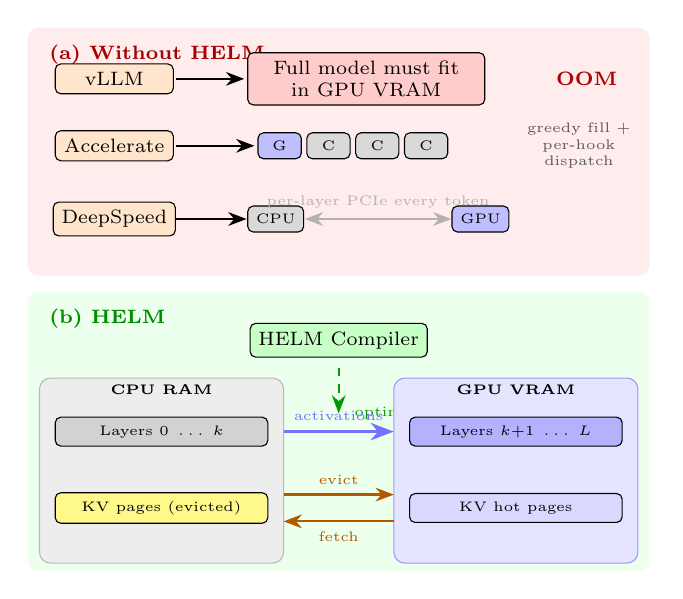
\begin{tikzpicture}[
  sbox/.style={draw, rounded corners=2pt, inner sep=3pt,
               font=\scriptsize, text centered},
  >=Stealth
]

%─── Panel A: Without HELM ────────────────────────────────────────────────
\fill[red!7, rounded corners=4pt] (0,0) rectangle (7.9,3.15);
\node[font=\scriptsize\bfseries, text=red!65!black, anchor=north west]
  at (0.15,3.05) {(a) Without HELM};

% vLLM
\node[sbox, fill=orange!20, minimum width=1.5cm] at (1.1,2.50) {vLLM};
\node[sbox, fill=red!20, minimum width=3.0cm, text width=2.8cm]
  at (4.3,2.50) {Full model must fit\\in GPU VRAM};
\draw[->, thick] (1.88,2.50) -- (2.75,2.50);
\node[font=\scriptsize\bfseries, text=red!70!black] at (7.1,2.50) {\textbf{OOM}};

% Accelerate
\node[sbox, fill=orange!20, minimum width=1.5cm] at (1.1,1.65) {Accelerate};
\node[sbox, fill=blue!25,  minimum width=0.55cm, font=\tiny] at (3.2,1.65) {G};
\node[sbox, fill=gray!30,  minimum width=0.55cm, font=\tiny] at (3.82,1.65) {C};
\node[sbox, fill=gray!30,  minimum width=0.55cm, font=\tiny] at (4.44,1.65) {C};
\node[sbox, fill=gray!30,  minimum width=0.55cm, font=\tiny] at (5.06,1.65) {C};
\draw[->, thick] (1.88,1.65) -- (2.88,1.65);
\node[font=\tiny, text width=1.7cm, align=center, text=gray!70!black]
  at (7.0,1.65) {greedy fill +\\per-hook dispatch};

% DeepSpeed
\node[sbox, fill=orange!20, minimum width=1.5cm] at (1.1,0.72) {DeepSpeed};
\node[sbox, fill=gray!30, minimum width=0.65cm, font=\tiny] at (3.15,0.72) {CPU};
\node[sbox, fill=blue!25, minimum width=0.65cm, font=\tiny] at (5.75,0.72) {GPU};
\draw[->, thick] (1.88,0.72) -- (2.78,0.72);
\draw[<->, thick, gray!60] (3.52,0.72) -- node[above, font=\tiny]
  {per-layer PCIe every token} (5.38,0.72);

%─── Panel B: HELM ────────────────────────────────────────────────────────
\fill[green!7, rounded corners=4pt] (0,-3.75) rectangle (7.9,-0.20);
\node[font=\scriptsize\bfseries, text=green!55!black, anchor=north west]
  at (0.15,-0.30) {(b) HELM};

% Compiler box
\node[sbox, fill=green!22, minimum width=2.1cm] (comp) at (3.95,-0.82)
  {HELM Compiler};
\draw[->, dashed, green!60!black, thick] (3.95,-1.17) -- (3.95,-1.75)
  node[right, font=\tiny, xshift=2pt] {optimal $k$};

% CPU block
\draw[fill=gray!14, draw=gray!55, rounded corners=4pt]
  (0.15,-3.65) rectangle (3.25,-1.30);
\node[font=\tiny\bfseries] at (1.70,-1.45) {CPU RAM};
\node[sbox, fill=gray!35, minimum width=2.7cm, font=\tiny]
  at (1.70,-1.98) {Layers $0 \;\ldots\; k$};
\node[sbox, fill=yellow!45, minimum width=2.7cm, font=\tiny]
  at (1.70,-2.95) {KV pages (evicted)};

% GPU block
\draw[fill=blue!10, draw=blue!40, rounded corners=4pt]
  (4.65,-3.65) rectangle (7.75,-1.30);
\node[font=\tiny\bfseries] at (6.20,-1.45) {GPU VRAM};
\node[sbox, fill=blue!30, minimum width=2.7cm, font=\tiny]
  at (6.20,-1.98) {Layers $k{+}1 \;\ldots\; L$};
\node[sbox, fill=blue!15, minimum width=2.7cm, font=\tiny]
  at (6.20,-2.95) {KV hot pages};

% Activation arrow (single PCIe transfer)
\draw[->, very thick, blue!55] (3.25,-1.98) --
  node[above, font=\tiny] {activations} (4.65,-1.98);

% KV evict / fetch arrows
\draw[->, thick, orange!70!black] (3.25,-2.78) --
  node[above, font=\tiny] {evict} (4.65,-2.78);
\draw[<-, thick, orange!70!black] (3.25,-3.12) --
  node[below, font=\tiny] {fetch} (4.65,-3.12);

\end{tikzpicture}
\caption{(a)~vLLM fails on sub-16\,GB GPUs; Accelerate's greedy layer
assignment is sub-optimal and uses slow per-hook dispatch; DeepSpeed incurs
$O(L)$ PCIe round-trips per generated token.
(b)~HELM's roofline cost model selects the optimal layer split~$k$, compiles
static per-device subgraphs (only \emph{activations} cross PCIe once per
step), and pages KV to CPU RAM for context lengths beyond GPU VRAM capacity.}
\label{fig:motivation}
\end{figure}

% ─────────────────────────────────────────────────────────────────────────────
\section{Introduction}
\label{sec:intro}
\IEEEPARstart{T}{he} parameters of state-of-the-art large language models
have grown from billions to hundreds of billions over the past three years.
A full-precision (fp16) copy of a 7\,B-parameter model occupies
$\approx$\,14\,GB; a 70\,B model requires $\approx$\,140\,GB; and mixture-of-experts
architectures store far more parameters than are active per token. Consumer GPUs
(RTX~4060, 8\,GB) and prosumer GPUs (RTX~3090, 24\,GB) cannot hold these
weights entirely in VRAM.

The practical consequences are severe. A researcher with a single 8\,GB GPU
and 32\,GB of CPU RAM cannot run a 7\,B model at all with vLLM, which requires
the entire model to reside in GPU memory before it accepts requests. She could
use HuggingFace Accelerate's \texttt{device\_map=`auto'}, which
fills GPU layers greedily from the first layer and spills the rest to CPU, but
Accelerate attaches per-module forward hooks and moves activations one module
at a time, achieving throughput well below the bandwidth-limited theoretical
maximum. FlexGen~\cite{flexgen} streams weights from CPU or disk during
inference, which amortizes data-movement cost only at batch sizes of hundreds ---
impractical for interactive use. DeepSpeed ZeRO-Inference~\cite{deepspeed}
moves one layer at a time to GPU for each forward pass, incurring per-layer
PCIe transfer overhead on every token.

What is missing is a system that (a) determines \emph{analytically}, before
generating any tokens, which partition of the model across CPU and GPU
minimises the latency objective on the specific hardware available, and (b)
executes that partition efficiently without per-token weight movement.
Fig.~\ref{fig:motivation} illustrates the problem and HELM's approach.

We present \textbf{HELM} (Heterogeneous Execution for Large Models), which
takes exactly this approach. The core insight is that the optimal CPU$\to$GPU
split is predictable from three quantities: the hardware's measured bandwidth
and FLOPS (for the specific regime --- decode at batch=1 is memory-bound;
prefill at large sequence length is compute-bound), the model's parameter
and KV-cache bytes per block, and the inter-device PCIe bandwidth. These
quantities can be measured in a $<$1\,s microbenchmark, and the optimal
partition can be found by scoring all $O(N)$ feasible splits under a
roofline cost model --- a one-time compile step.

The resulting system offers three properties that existing tools do not
simultaneously provide:

\begin{itemize}
  \item \textbf{Fit guarantee.} HELM loads models that exceed GPU VRAM by
        placing layers on CPU as needed, with a VRAM feasibility check that
        correctly excludes KV-cache pages when KV offload is enabled.
  \item \textbf{Optimal throughput for the available hardware.} The
        hardware-calibrated roofline model selects the partition that
        minimises decode latency, avoiding the greedy ``fill GPU from layer 0''
        assumption that leaves GPU bandwidth underutilised.
  \item \textbf{Unbounded context.} The paged KV-cache offload manager
        evicts cold pages to CPU RAM and streams them back on demand,
        decoupling context length from VRAM capacity.
\end{itemize}

This paper makes the following contributions:

\begin{enumerate}
  \item A \textbf{compiler pipeline} that traces an \texttt{nn.Module} into
        two FX graphs (prefill and decode), annotates each transformer block
        with hardware-measured costs, and compiles the optimal CPU$\to$GPU
        split into standalone per-device subgraphs executed without
        per-token weight movement (\S\ref{sec:overview}, \S\ref{sec:strategy}).
  \item A \textbf{hardware-calibrated roofline cost model} with separate
        projection and attention sub-rooflines, an L3 cache model for
        short-context KV traffic, and GQA-aware KV byte accounting.
        An exhaustive $O(L)$ search over all feasible splits returns the
        globally optimal partition in $<$1\,ms (\S\ref{sec:costmodel}).
  \item A \textbf{paged KV-cache manager} with a per-GPU watermark,
        async H2D prefetch, and page-streaming online softmax that
        decouples context length from VRAM capacity (\S\ref{sec:kv}).
  \item An \textbf{end-to-end evaluation} across 3 hardware
        configurations and 4 model sizes from 4\,B to 32\,B parameters,
        comparing HELM against vLLM, HuggingFace Accelerate, and DeepSpeed
        ZeRO-Inference (\S\ref{sec:eval}).
\end{enumerate}

% ─────────────────────────────────────────────────────────────────────────────
\section{Background and Related Work}
\label{sec:related}

\subsection{LLM Inference Regimes}

Transformer~\cite{attention} inference proceeds in two phases. During
\emph{prefill}, all input tokens are processed simultaneously: the dominant
operation is matrix multiplication at shape $(S, H) \times (H, H)$, which
for large $S$ achieves high arithmetic intensity and is compute-bound on
modern GPUs. During \emph{decode}, a single new token is generated per step:
the dominant operation is a matrix-vector product at shape $(1, H) \times
(H, H)$, which has arithmetic intensity of $\approx 1$\,FLOP/byte and is
memory-bandwidth-bound on all current hardware~\cite{roofline}.

This distinction matters for partitioning. A CPU stage is tolerable for
prefill (it is a one-time cost proportional to input length) but damaging
for decode (it executes once per output token). HELM's cost model accounts
for both regimes separately.

\subsection{Memory-Constrained Inference}

\textbf{llama.cpp}~\cite{llamacpp} quantises weights to 2--8 bits (GGUF
format) and supports partial GPU offload via the \texttt{--n-gpu-layers}
parameter. However, the layer count must be tuned manually; there is no
analytical cost model to determine the optimal split, and the unquantised
fp16 path is CPU-only.

\textbf{HuggingFace Accelerate}~\cite{accelerate} implements
\texttt{device\_map=`auto'}, which assigns layers to devices in order,
filling GPU VRAM before spilling to CPU. It uses dispatch hooks that execute
device transfers inside every module forward pass, introducing Python-level
synchronisation at each layer boundary.

\textbf{DeepSpeed ZeRO-Inference}~\cite{deepspeed} partitions parameters
across CPU and GPU at the tensor level and fetches each layer's weights to
GPU just before the forward pass. This is effective for large batch sizes but
incurs $O(L)$ PCIe round-trips per generated token, where $L$ is the number
of layers.

\textbf{FlexGen}~\cite{flexgen} is designed for offline throughput at batch
sizes of $\sim$100--1000. It optimises a disk$\to$CPU$\to$GPU weight and
activation schedule. At batch=1 its design provides no advantage and its
scheduling overhead dominates.

\textbf{vLLM}~\cite{vllm} achieves high GPU utilisation via PagedAttention
and continuous batching but requires all model weights to fit in GPU VRAM at
load time. It has no facility for CPU-resident layers.

\textbf{Splitwise}~\cite{splitwise} and PipeSwitch~\cite{pipeswitch} split
prefill and decode phases across different GPU servers; they target
multi-GPU data-centre deployments, not single-node heterogeneous execution.

\subsection{Roofline Modelling}

The roofline model~\cite{roofline} characterises an operation's performance
as the maximum of its compute-bound and memory-bandwidth-bound ceilings:
$T = \max\!\left(F / P,\ B / M\right)$ where $F$ is FLOP count, $P$ is peak
FLOPS, $B$ is byte traffic, and $M$ is memory bandwidth. HELM applies this
model at the transformer-block granularity with hardware parameters measured
by runtime microbenchmarks rather than manufacturer specifications, avoiding
the gap between peak and achievable throughput.

\subsection{Graph Compilation for LLMs}

TensorRT-LLM~\cite{trtllm} and torch.compile~\cite{torchcompile} optimise
within a single device. They do not address cross-device partitioning.
AlpaServe~\cite{alphaserve} uses integer programming to partition transformer
layers across multiple GPUs in a cluster; HELM applies a similar philosophy
to the single-node CPU+GPU setting with an analytical (rather than ILP) cost
model that executes in microseconds.

% ─────────────────────────────────────────────────────────────────────────────
\section{System Overview}
\label{sec:overview}

Fig.~\ref{fig:pipeline} illustrates the HELM compilation and execution pipeline.
Given an \texttt{nn.Module} and a target workload description, HELM produces
two compiled artifacts --- a \emph{prefill graph} and a \emph{decode graph}
--- each split into per-device subgraphs that the PipelineRuntime executes
in sequence.
Fig.~\ref{fig:memory_timeline} shows the resulting memory layout and per-token
decode timeline for a representative Qwen3-8B deployment on an 8\,GB GPU.

\begin{figure*}[!t]
\centering
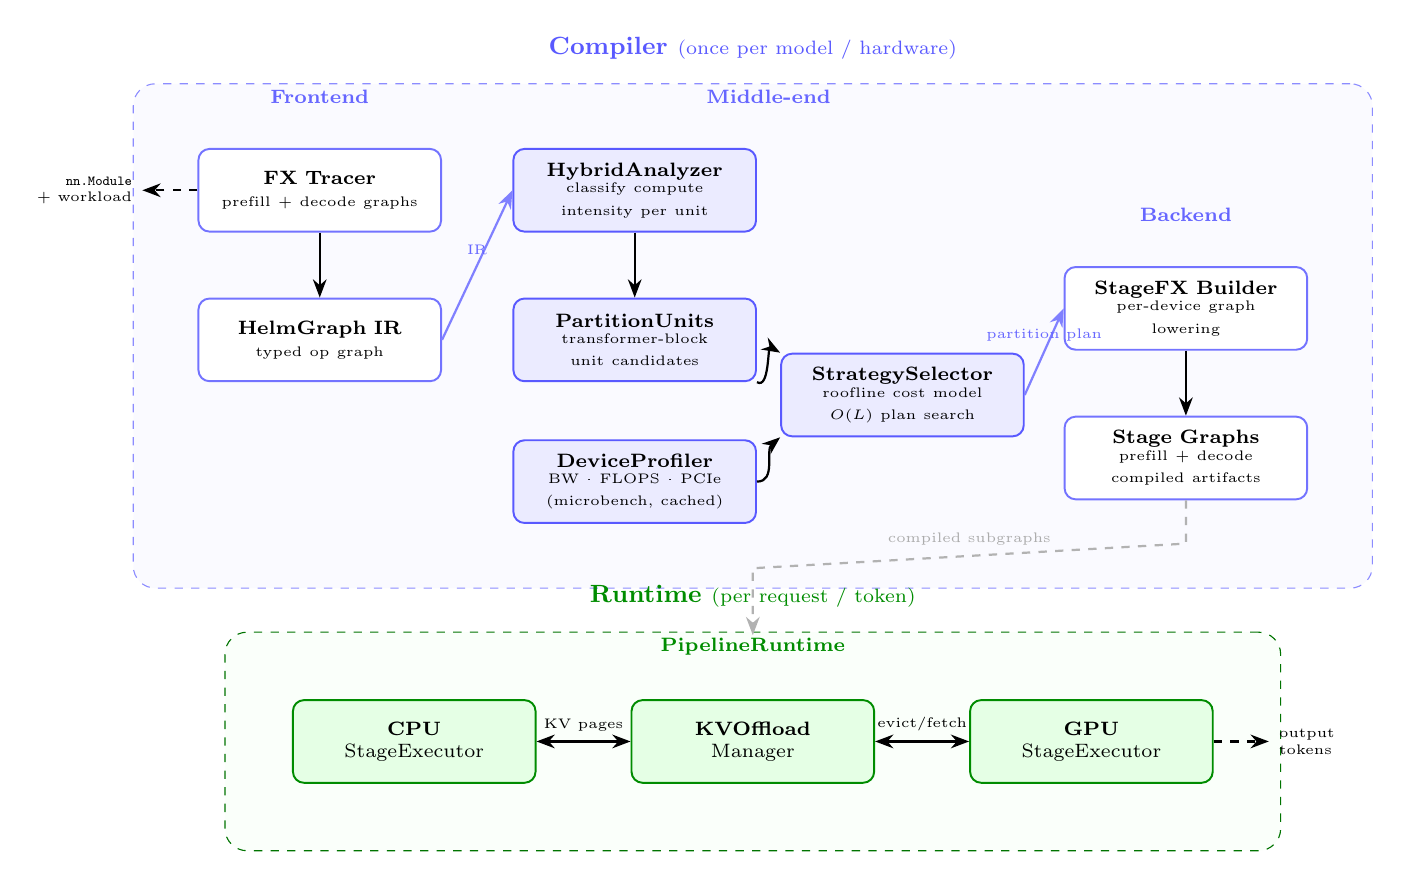
\begin{tikzpicture}[
  %% compile-time component box
  cbox/.style={draw=blue!55, fill=white, rounded corners=4pt,
               minimum height=1.05cm, minimum width=3.0cm,
               text centered, font=\scriptsize, text width=2.8cm,
               inner sep=4pt, line width=0.7pt},
  %% middle-end box (slightly tinted to stand out)
  mbox/.style={draw=blue!65, fill=blue!8, rounded corners=4pt,
               minimum height=1.05cm, minimum width=3.0cm,
               text centered, font=\scriptsize, text width=2.8cm,
               inner sep=4pt, line width=0.7pt},
  %% runtime component box
  rbox/.style={draw=green!55!black, fill=green!10, rounded corners=4pt,
               minimum height=1.05cm, minimum width=3.0cm,
               text centered, font=\scriptsize, text width=2.8cm,
               inner sep=4pt, line width=0.7pt},
  >=Stealth, thick, line width=0.8pt
]

%% ═══════════════════════════════════════════════════════════════════════════
%%  FRONTEND  (left column, x ≈ 1.8)
%% ═══════════════════════════════════════════════════════════════════════════
\node[cbox] (tracer) at (1.8,  0.0) {\textbf{FX Tracer}\\{\tiny prefill + decode graphs}};
\node[cbox] (ir)     at (1.8, -1.9) {\textbf{HelmGraph IR}\\{\tiny typed op graph}};
\draw[->] (tracer) -- (ir);

%% ═══════════════════════════════════════════════════════════════════════════
%%  MIDDLE-END  (centre, x ≈ 5.8 – 9.2)
%% ═══════════════════════════════════════════════════════════════════════════
\node[mbox] (hybrid)   at (5.8,  0.0) {\textbf{HybridAnalyzer}\\{\tiny classify compute\\intensity per unit}};
\node[mbox] (punits)   at (5.8, -1.9) {\textbf{PartitionUnits}\\{\tiny transformer-block\\unit candidates}};
\node[mbox] (profiler) at (5.8, -3.7) {\textbf{DeviceProfiler}\\{\tiny BW · FLOPS · PCIe\\(microbench, cached)}};
\node[mbox] (strategy) at (9.2, -2.6) {\textbf{StrategySelector}\\{\tiny roofline cost model\\$O(L)$ plan search}};

\draw[->] (hybrid) -- (punits);
\draw[->] (punits.south east)  to[out=-30, in=150] (strategy.north west);
\draw[->] (profiler.east)      to[out=0,   in=220] (strategy.south west);

%% ═══════════════════════════════════════════════════════════════════════════
%%  BACKEND  (right column, x ≈ 12.8)
%% ═══════════════════════════════════════════════════════════════════════════
\node[cbox] (builder) at (12.8, -1.5) {\textbf{StageFX Builder}\\{\tiny per-device graph\\lowering}};
\node[cbox] (stages)  at (12.8, -3.4) {\textbf{Stage Graphs}\\{\tiny prefill + decode\\compiled artifacts}};
\draw[->] (builder) -- (stages);

%% ═══════════════════════════════════════════════════════════════════════════
%%  CROSS-PHASE DATA FLOW
%% ═══════════════════════════════════════════════════════════════════════════
%% Frontend → Middle-end
\draw[->, blue!50] (ir.east)
  -- node[above, font=\tiny, text=blue!60] {IR}
  (hybrid.west);
%% Middle-end → Backend
\draw[->, blue!50] (strategy.east)
  -- node[above, font=\tiny, text=blue!60] {partition plan}
  (builder.west);

%% ═══════════════════════════════════════════════════════════════════════════
%%  INPUT
%% ═══════════════════════════════════════════════════════════════════════════
\draw[->, dashed] (tracer.west) -- ++(-0.7, 0)
  node[left, font=\tiny, align=right] {\texttt{nn.Module}\\+ workload};

%% ═══════════════════════════════════════════════════════════════════════════
%%  COMPILE → RUNTIME HANDOFF
%% ═══════════════════════════════════════════════════════════════════════════
\draw[->, dashed, gray!60, line width=0.8pt]
  (stages.south) -- ++(0, -0.55)
  -- node[above, font=\tiny, text=gray!65] {compiled subgraphs}
  (7.3, -4.8)
  -- (7.3, -5.65);

%% ═══════════════════════════════════════════════════════════════════════════
%%  RUNTIME  (PipelineRuntime contains three peers)
%% ═══════════════════════════════════════════════════════════════════════════
\node[rbox] (cpu) at ( 3.0, -7.0) {\textbf{CPU}\\StageExecutor};
\node[rbox] (kv)  at ( 7.3, -7.0) {\textbf{KVOffload}\\Manager};
\node[rbox] (gpu) at (11.6, -7.0) {\textbf{GPU}\\StageExecutor};

\draw[<->] (cpu) -- node[above, font=\tiny] {KV pages}    (kv);
\draw[<->] (kv)  -- node[above, font=\tiny] {evict/fetch} (gpu);

%% Output
\draw[->, dashed] (gpu.east) -- ++(0.7, 0)
  node[right, font=\tiny, align=left] {output\\tokens};

%% ═══════════════════════════════════════════════════════════════════════════
%%  BACKGROUND REGIONS  (drawn last so node names are resolved)
%% ═══════════════════════════════════════════════════════════════════════════
\begin{scope}[on background layer]
  %% phase sub-regions
  \node[fill=blue!5,  draw=blue!25, rounded corners=5pt, inner sep=9pt,
        fit=(tracer)(ir)]                              (fe) {};
  \node[fill=blue!11, draw=blue!40, rounded corners=5pt, inner sep=9pt,
        fit=(hybrid)(punits)(profiler)(strategy)]      (me) {};
  \node[fill=blue!5,  draw=blue!25, rounded corners=5pt, inner sep=9pt,
        fit=(builder)(stages)]                         (be) {};
  %% compiler outer region
  \node[fill=blue!2, draw=blue!45, rounded corners=8pt,
        dashed, inner sep=14pt, fit=(fe)(me)(be)]      (compiler) {};
  %% PipelineRuntime inner container
  \node[fill=green!7, draw=green!50!black, rounded corners=5pt, inner sep=10pt,
        fit=(cpu)(kv)(gpu)]                            (prt) {};
  %% runtime outer region
  \node[fill=green!2, draw=green!45!black, rounded corners=8pt,
        dashed, inner sep=14pt, fit=(prt)]             (runtime) {};
\end{scope}

%% ═══════════════════════════════════════════════════════════════════════════
%%  LABELS  (placed after background so they render on top)
%% ═══════════════════════════════════════════════════════════════════════════
%% phase headers inside compiler region
\node[above=3pt of fe, font=\scriptsize\bfseries, text=blue!60] {Frontend};
\node[above=3pt of me, font=\scriptsize\bfseries, text=blue!60] {Middle-end};
\node[above=3pt of be, font=\scriptsize\bfseries, text=blue!60] {Backend};
%% region titles
\node[above=5pt of compiler, font=\small\bfseries, text=blue!65]
  {Compiler \normalfont\scriptsize(once per model / hardware)};
\node[above=5pt of runtime,  font=\small\bfseries, text=green!55!black]
  {Runtime \normalfont\scriptsize(per request / token)};
%% PipelineRuntime label inside the green container
\node[above=2pt of prt, font=\scriptsize\bfseries, text=green!55!black]
  {PipelineRuntime};

\end{tikzpicture}
\caption{HELM compiler and runtime architecture.
The \textbf{Frontend} traces the \texttt{nn.Module} into a typed HelmGraph IR.
The \textbf{Middle-end} classifies arithmetic intensity per partition unit,
microbenchmarks hardware (DRAM bandwidth, FLOPS, PCIe; results cached), and
exhaustively scores all $O(L)$ feasible CPU$\to$GPU split points under the
roofline cost model (\S\ref{sec:costmodel}).
The \textbf{Backend} lowers the chosen partition plan into per-device
\texttt{torch.fx} stage graphs (one prefill graph, one decode graph per device).
At runtime the \textbf{PipelineRuntime} sequences the CPU and GPU
\textbf{StageExecutors}; the \textbf{KVOffload Manager} evicts cold KV-cache
pages to CPU pinned RAM when the GPU watermark is exceeded.}
\label{fig:pipeline}
\end{figure*}

The pipeline consists of ten stages:

\textbf{(1) FX Tracing.} HELM captures two \texttt{torch.fx.GraphModule}
objects. The \emph{prefill graph} processes the full input sequence at once;
the dominant operation is matrix multiplication at shape $(S, H) \times
(H, H)$, which is compute-bound at large $S$. The \emph{decode graph}
processes a single new token per step against a pre-built KV cache; the
dominant operation is a matrix-vector product at shape $(1, H) \times (H,
H)$, which is memory-bandwidth-bound. Separate graphs are necessary because
the two regimes have different arithmetic intensities, different attention
implementations (full SDPA for prefill vs.\ cached-KV for decode), and
therefore different optimal partitions. Both graphs are captured via symbolic
tracing with fallback to concrete tracing for models that use dynamic control
flow.

\textbf{(2) HelmGraph IR.} FX nodes are lifted into a typed intermediate
representation that annotates each node with its inferred shape, estimated
FLOP count, and estimated parameter bytes.
FX alone is insufficient for partition decisions: a raw \texttt{torch.fx.Node}
carries no shape, no FLOP count, and no byte-cost information, so it cannot
be fed to a roofline cost model.
Fig.~\ref{fig:ir_comparison} shows the contrast between an FX node and its
HelmGraph IR counterpart, and how the IR annotations aggregate into a
scored \emph{PartitionUnit}.

\textbf{(3) HybridAnalyzer.} A static pass over the IR annotates each
transformer block with three quantities: $W_\text{param}$ (parameter bytes
read per token), $W_\text{act}$ (activation bytes crossing the inter-stage
boundary), and $W_\text{kv}$ (KV-cache bytes accessed per decode step).

\textbf{(4) PartitionUnitBuilder.} The IR is grouped into coarse
\emph{partition units}: one embedding unit, $L$ transformer-block units
(one per layer), and one output-projection unit.

% ── FX vs HelmIR comparison figure ──────────────────────────────────────────
\begin{figure*}[!t]
\centering
\newcommand{\kf}[1]{\makebox[1.55cm][l]{\texttt{#1}}}% key field, fixed width
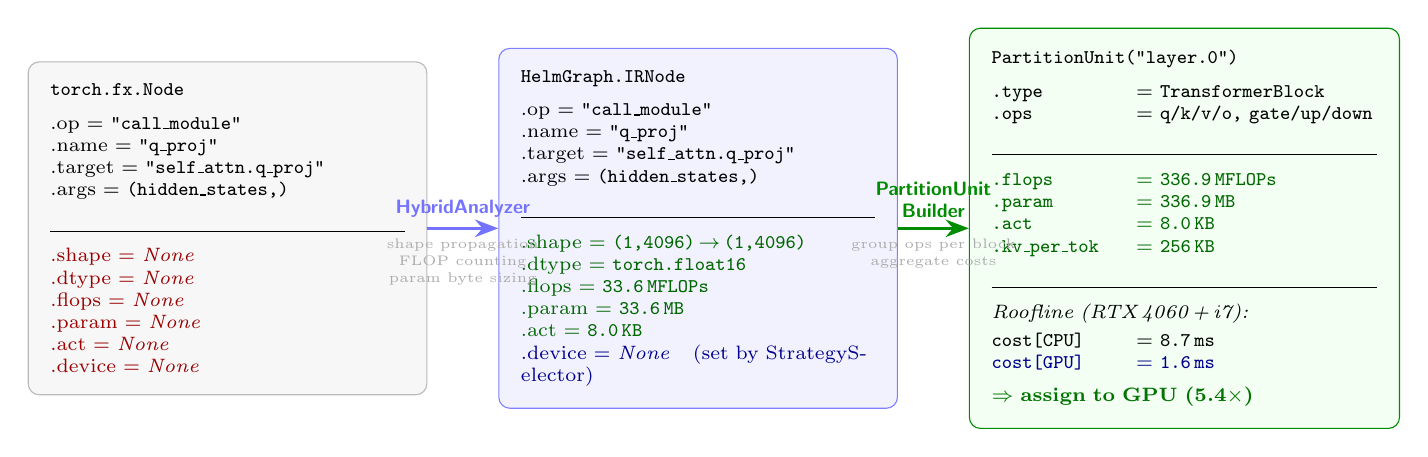
\begin{tikzpicture}[
  >=Stealth,
  fxbox/.style={draw=gray!55, fill=gray!6, rounded corners=4pt,
                inner sep=8pt, text width=4.5cm, align=left,
                font=\ttfamily\scriptsize},
  irbox/.style={draw=blue!50, fill=blue!5, rounded corners=4pt,
                inner sep=8pt, text width=4.5cm, align=left,
                font=\ttfamily\scriptsize},
  pubox/.style={draw=green!55!black, fill=green!5, rounded corners=4pt,
                inner sep=8pt, text width=4.9cm, align=left,
                font=\ttfamily\scriptsize},
]

%── Panel 1: raw torch.fx.Node ───────────────────────────────────────────────
\node[fxbox] (fx) {%
  \normalfont\textbf{\texttt{torch.fx.Node}}\\[4pt]
  \kf{.op}     = \texttt{"call\_module"}\\
  \kf{.name}   = \texttt{"q\_proj"}\\
  \kf{.target} = \texttt{"self\_attn.q\_proj"}\\
  \kf{.args}   = \texttt{(hidden\_states,)}\\[5pt]
  \rule{\linewidth}{0.25pt}\\[3pt]
  {\color{red!60!black}%
  \kf{.shape}  = \textit{None}\\
  \kf{.dtype}  = \textit{None}\\
  \kf{.flops}  = \textit{None}\\
  \kf{.param}  = \textit{None}\\
  \kf{.act}    = \textit{None}\\
  \kf{.device} = \textit{None}}%
};

%── Panel 2: HelmGraph.IRNode ────────────────────────────────────────────────
\node[irbox, right=0.9cm of fx] (helm) {%
  \normalfont\textbf{\texttt{HelmGraph.IRNode}}\\[4pt]
  \kf{.op}     = \texttt{"call\_module"}\\
  \kf{.name}   = \texttt{"q\_proj"}\\
  \kf{.target} = \texttt{"self\_attn.q\_proj"}\\
  \kf{.args}   = \texttt{(hidden\_states,)}\\[5pt]
  \rule{\linewidth}{0.25pt}\\[3pt]
  {\color{green!40!black}%
  \kf{.shape}  = \texttt{(1,4096)\,$\to$\,(1,4096)}\\
  \kf{.dtype}  = \texttt{torch.float16}\\
  \kf{.flops}  = \texttt{33.6\,MFLOPs}\\
  \kf{.param}  = \texttt{33.6\,MB}\\
  \kf{.act}    = \texttt{8.0\,KB}}\\
  {\color{blue!55!black}\kf{.device} = \textit{None}\quad\normalfont\textnormal{\scriptsize(set by StrategySelector)}}%
};

%── Panel 3: PartitionUnit ───────────────────────────────────────────────────
\newcommand{\kp}[1]{\makebox[1.75cm][l]{\texttt{#1}}}% key field for pu panel
\node[pubox, right=0.9cm of helm] (pu) {%
  \normalfont\textbf{\texttt{PartitionUnit("layer.0")}}\\[4pt]
  \kp{.type}   = \texttt{TransformerBlock}\\
  \kp{.ops}    = \texttt{q/k/v/o, gate/up/down}\\[5pt]
  \rule{\linewidth}{0.25pt}\\[3pt]
  {\color{green!40!black}%
  \kp{.flops}  = \texttt{336.9\,MFLOPs}\\
  \kp{.param}  = \texttt{336.9\,MB}\\
  \kp{.act}    = \texttt{8.0\,KB}\\
  \kp{.kv\_per\_tok} = \texttt{256\,KB}}\\[5pt]
  \rule{\linewidth}{0.25pt}\\[3pt]
  \normalfont\textit{\scriptsize Roofline (RTX\,4060\,+\,i7):}\\[2pt]
  \kp{cost[CPU]} = \texttt{8.7\,ms}\\
  {\color{blue!55!black}\kp{cost[GPU]} = \texttt{1.6\,ms}}\\[4pt]
  {\color{green!45!black}\normalfont\bfseries $\Rightarrow$ assign to GPU\;(5.4$\times$)}%
};

%── Arrows ───────────────────────────────────────────────────────────────────
\draw[->, very thick, blue!55] (fx.east) -- (helm.west)
  node[pos=0.5, above, font=\scriptsize\bfseries\sffamily, align=center]
    {HybridAnalyzer}
  node[pos=0.5, below, font=\tiny\rmfamily, text=gray!65, align=center]
    {shape propagation\\FLOP counting\\param byte sizing};

\draw[->, very thick, green!55!black] (helm.east) -- (pu.west)
  node[pos=0.5, above, font=\scriptsize\bfseries\sffamily, align=center]
    {PartitionUnit\\Builder}
  node[pos=0.5, below, font=\tiny\rmfamily, text=gray!65, align=center]
    {group ops per block\\aggregate costs};

\end{tikzpicture}
\caption{%
\textbf{From raw FX node to scored PartitionUnit.}
A \texttt{torch.fx.Node} (\emph{left}) carries no shape, dtype, FLOP count,
or byte-cost information.
The \emph{HybridAnalyzer} lifts each node into a \texttt{HelmGraph.IRNode}
(\emph{centre}) by running shape propagation and FLOP/byte estimation;
\texttt{.device} remains unassigned until StrategySelector runs.
The \emph{PartitionUnitBuilder} groups all IR nodes for one transformer block
into a \texttt{PartitionUnit} (\emph{right}) with block-level totals.
The StrategySelector then evaluates the roofline cost model (Alg.~\ref{alg:strategy})
for each device and selects the assignment minimising $T_\text{plan}$.
Numbers shown for Qwen3-8B on RTX~4060\,+\,Intel Core i7
(CPU DRAM: 40\,GB/s; GPU effective BW: 218\,GB/s).}
\label{fig:ir_comparison}
\end{figure*}

\textbf{(5) DeviceProfiler.} Three microbenchmarks run once per process:
(i) a 64\,MB tensor copy to measure peak memory bandwidth; (ii) for
CPU decode-regime FLOPS, the profiler sets effective FLOPS~$=$~DRAM
bandwidth, because HELM's AVX2+F16C kernel makes CPU GEMV
memory-bandwidth-bound ($\approx$1\,FLOP/byte) and PyTorch's CPU
fp16 matmul has no AVX2 BLAS path; (iii) a $(128, H) \times (H, H)$
fp32 GEMM to measure prefill-regime FLOPS (fp16 weights are upcast
to fp32 on x86 during the forward pass).
Two additional PCIe benchmarks measure H2D and D2H transfer rates using
pinned host memory. Results are cached across \texttt{compile()} calls.

\textbf{(6) StrategySelector.} Given the partition units and hardware
profiles, the selector evaluates every feasible assignment of consecutive
blocks to CPU and GPU (a single CPU$\to$GPU stage boundary), scores each
assignment with the roofline cost model, and returns the plan minimising
the configured objective (decode latency, prefill latency, or throughput).

\textbf{(7) StageFXBuilder.} The chosen plan is used to split the FX graph
into per-stage \texttt{GraphModule} objects, each runnable on its assigned
device as a standalone function.

\textbf{(8) PipelineRuntime.} Orchestrates the prefill loop (single forward
pass through both stages) and the autoregressive decode loop (one
decode-graph forward pass per generated token). Supports $\text{batch\_size} \geq 1$.

\textbf{(9) StageRuntimeExecutor.} Executes stages in sequence, moving the
activation tensor across the device boundary after each stage. Before the
first request, weights are pre-positioned to their target devices one
submodule at a time, avoiding the spike of holding the full model in CPU RAM
simultaneously during device transfer.

\textbf{(10) KVOffloadManager.} Maintains a paged KV cache shared across
batch items. When GPU VRAM usage exceeds a configurable watermark, it evicts
the oldest page to CPU RAM and streams it back during attention computation.

% ─────────────────────────────────────────────────────────────────────────────
\section{Hardware-Calibrated Cost Model}
\label{sec:costmodel}

\subsection{Device and Link Profiles}

The DeviceProfiler produces a \emph{DeviceProfile} for each available device:
\begin{equation}
  \mathcal{D} = (P_\text{dec},\ P_\text{pre},\ M,\ C_\text{L3},\ B_\text{L3})
\end{equation}
where $P_\text{dec}$ and $P_\text{pre}$ are the measured effective FLOPS in
the decode and prefill regimes respectively, $M$ is DRAM bandwidth,
$C_\text{L3}$ is L3 cache size (CPU only), and $B_\text{L3}$ is L3 bandwidth
(estimated as $3\times$ DRAM bandwidth). A \emph{LinkProfile}
$\mathcal{L} = (B_\text{link}, \ell)$ records the bandwidth and latency of
each device-to-device path (PCIe H2D and D2H).

\subsection{Per-Stage Decode Time}

For a stage assigned to device $\mathcal{D}$, processing a batch of $B$
requests with context length $c$, the estimated decode time per generated
token is:
\begin{equation}
  T_\text{decode} = T_\text{proj} + T_\text{attn} + T_\text{comm}
  \label{eq:decode}
\end{equation}

The \emph{projection term} accounts for all linear layers in the block (QKV
projections, output projection, and both MLP projections):
\begin{align}
  F_\text{proj} &= 2B\!\left(2H^2 + 2H d_\text{kv} + H I + I H + H I\right) \cdot n_\ell
  \label{eq:fprojdec}\\
  T_\text{proj} &= \max\!\left(\frac{F_\text{proj}}{P_\text{dec}\,\eta_c},\
                               \frac{W_\text{param}}{M\,\eta_m}\right)
  \label{eq:tproj}
\end{align}
where $H$ is hidden size, $d_\text{kv} = h_\text{kv} d_h$ is the KV
projection dimension, $I$ is intermediate (MLP) size, $n_\ell$ is the
number of blocks in the stage, and $\eta_c, \eta_m \in (0,1]$ are hardware
efficiency coefficients.

The \emph{attention term} uses the effective KV bandwidth $\hat{M}$, which
accounts for L3 cache residency at short contexts (CPU only):
\begin{align}
  F_\text{attn} &= 4B\,h_a\,c\,d_h \cdot n_\ell
  \label{eq:fattndec}\\
  W_\text{kv}  &= 2 \cdot 2\,B\,n_\ell\,c\,h_\text{kv}\,d_h\,d_\text{sz}
  \label{eq:wkv}\\
  T_\text{attn} &= \max\!\left(\frac{F_\text{attn}}{P_\text{dec}\,\eta_c},\
                               \frac{W_\text{kv}}{\hat{M}\,\eta_m}\right)
  \label{eq:tattn}
\end{align}
where $h_a$ is the number of attention heads, $h_\text{kv} \leq h_a$ is the
number of KV heads (supporting Grouped-Query Attention~\cite{gqa} where
$h_\text{kv} < h_a$ reduces KV cache size by $h_a / h_\text{kv}$), $d_h$
is head dimension, and $d_\text{sz}$ is bytes per element.
On GPU, FlashAttention tiles $Q$, $K$, $V$ in SRAM so no intermediate
$QK^\top$ tensors are written to HBM; however, $K$ and $V$ are still
\emph{read} from HBM, so $W_\text{kv}$ remains and both roofline terms
in~\eqref{eq:tattn} apply unchanged.

\subsection{L3 Cache Hierarchy}

At short context lengths, the KV working set fits in the CPU's L3 cache.
We model the effective KV bandwidth as a linear blend:
\begin{equation}
  \hat{M} = \alpha\,B_\text{L3} + (1-\alpha)\,M, \quad
  \alpha = \min\!\left(1,\ \frac{C_\text{L3}}{W_\text{kv}}\right)
  \label{eq:l3}
\end{equation}
As context grows, $\alpha \to 0$ and the effective bandwidth falls to DRAM
bandwidth. The L3 size $C_\text{L3}$ is queried from \texttt{cpuinfo} at
startup; the bandwidth $B_\text{L3}$ is estimated conservatively as
$3\times$ the measured DRAM bandwidth.

\subsection{Per-Stage Prefill Time}

The prefill term differs from decode in two ways: (i) sequence length $S$
replaces batch=1, and (ii) GPU activation traffic is zero because
FlashAttention keeps $Q$, $K$, $V$ tiles in SRAM throughout.

\begin{align}
  F^\text{pre}_\text{proj} &= 2BS\!\left(2H^2 + 2H d_\text{kv} + H I + IH + HI\right) \cdot n_\ell \\
  F^\text{pre}_\text{attn} &= 2B\,h_a\,S^2\,d_h \cdot n_\ell \\
  W^\text{pre}_\text{attn} &=
    \begin{cases}
      0 & \text{GPU (FlashAttention)} \\
      2\,B\,S\,H\,d_\text{sz} \cdot n_\ell & \text{CPU}
    \end{cases}\\
  T_\text{prefill} &= T^\text{pre}_\text{proj} + T^\text{pre}_\text{attn}
                      + T_\text{comm}
\end{align}

\subsection{Communication Cost}

Each stage boundary incurs one activation transfer of size
$W_\text{act} = B \cdot S_\text{cur} \cdot H \cdot d_\text{sz}$ bytes,
where $S_\text{cur} = 1$ during decode and $S_\text{cur} = S$ during
prefill:
\begin{equation}
  T_\text{comm} = \ell_\text{link} + \frac{W_\text{act}}{B_\text{link}}
  \label{eq:comm}
\end{equation}
For single-stage (all-GPU or all-CPU) plans, $T_\text{comm} = 0$.

\subsection{Plan Score and Objective}

Given a partition plan $\pi$ assigning $k$ blocks to CPU and $L-k$ blocks
to GPU, the plan cost is:
\begin{align}
  T_\text{plan}(\pi) &= T^\text{CPU}_\text{decode}(k) + T^\text{GPU}_\text{decode}(L-k)
                       + T_\text{comm} \label{eq:plan}
\end{align}
The StrategySelector evaluates (\ref{eq:plan}) for all $k \in \{0,\ldots,L\}$
subject to the GPU VRAM feasibility constraint:
\begin{equation}
  W_\text{param}(L-k) + \mathbf{1}_\text{kv-GPU} \cdot W_\text{kv}^\text{total}
  \leq \text{VRAM}_\text{avail}
  \label{eq:feasibility}
\end{equation}
The plan minimising $T_\text{plan}$ is selected. When
\texttt{kv\_offload=True}, $\mathbf{1}_\text{kv-GPU} = 0$ and the KV cache
does not count against the GPU budget.
Algorithm~\ref{alg:strategy} gives the complete procedure.

\begin{algorithm}[t]
\caption{StrategySelector: Exhaustive Roofline Partition Search}
\label{alg:strategy}
\begin{algorithmic}[1]
\REQUIRE Partition units $\{u_i\}_{i=0}^{L}$,
         device profiles $\mathcal{D}_\text{cpu}$, $\mathcal{D}_\text{gpu}$,
         link profile $\mathcal{L}$,
         $\mathrm{VRAM}_\text{avail}$,
         objective $\in \{\text{decode},\,\text{prefill}\}$
\ENSURE Optimal partition plan $\pi^{*}$
\STATE $\pi^{*} \leftarrow \bot$;\quad $T^{*} \leftarrow \infty$
\FOR{$k \leftarrow 0$ \textbf{to} $L$}
  \STATE $W_\text{gpu} \leftarrow \textstyle\sum_{i=k}^{L} u_i.\text{param\_bytes}$
  \IF{$W_\text{gpu} > \mathrm{VRAM}_\text{avail}$}
    \STATE \textbf{continue}
  \ENDIF
  \STATE $T_\text{cpu} \leftarrow \textsc{RooflineTime}(\{u_i\}_{i < k},\;\mathcal{D}_\text{cpu},\;\text{objective})$
  \STATE $T_\text{gpu} \leftarrow \textsc{RooflineTime}(\{u_i\}_{i \geq k},\;\mathcal{D}_\text{gpu},\;\text{objective})$
  \STATE $T_\text{comm} \leftarrow \mathcal{L}.\ell + u_k.\text{act\_bytes}\;/\;\mathcal{L}.B$
  \STATE $T_\text{plan} \leftarrow T_\text{cpu} + T_\text{gpu} + T_\text{comm}$
  \IF{$T_\text{plan} < T^{*}$}
    \STATE $T^{*} \leftarrow T_\text{plan}$;\quad
           $\pi^{*} \leftarrow (k,\;\mathcal{D}_\text{cpu},\;\mathcal{D}_\text{gpu})$
  \ENDIF
\ENDFOR
\RETURN $\pi^{*}$
\end{algorithmic}
\end{algorithm}

% ─────────────────────────────────────────────────────────────────────────────
\section{Partition Strategy and Compilation}
\label{sec:strategy}

\subsection{Exhaustive Split Search}

The StrategySelector evaluates three classes of plans:
(1) all-GPU, (2) all feasible CPU$\to$GPU 2-stage splits ($k = 1,\ldots,L-1$),
and (3) all-CPU. For each feasible plan the cost is scored using the roofline
model of \S\ref{sec:costmodel}. The minimum-cost feasible plan is returned.

This exhaustive search has $O(L)$ cost ($L \approx 28$--$80$ for current
models) and takes $<$1\,ms per query. The greedy ``first-feasible'' heuristic
used by prior systems (most GPU layers wins) fails when the GPU stage becomes
memory-bound before the CPU stage, causing the boundary communication term
to dominate --- a situation HELM's exhaustive search correctly handles.

\subsection{FX Graph Splitting}

Given the plan, the StageFXBuilder partitions the flat FX graph into a
sequence of per-stage \texttt{GraphModule} objects. Stage boundaries are
inserted after the last node belonging to the CPU stage; the activation
tensor at that point is annotated as a graph output/input pair. Each
subgraph is a standalone callable that can be compiled independently with
\texttt{torch.compile} or TorchScript.

Algorithm~\ref{alg:helm} summarises the full compile-and-execute flow.

\begin{algorithm}[t]
\caption{HELM: Heterogeneous Compile and Execute}
\label{alg:helm}
\begin{algorithmic}[1]
\REQUIRE $\mathcal{M}$: \texttt{nn.Module},
         workload $\mathcal{W}{=}(S, T_\text{out}, B)$,
         hardware $\mathcal{H}$
\ENSURE Token stream for input prompt
\vspace{2pt}
\textbf{Compile phase} \textnormal{(once per model\,/\,hardware pair)}
\STATE $(G_\text{pre},\,G_\text{dec}) \leftarrow \textsc{FXTrace}(\mathcal{M}, \mathcal{W})$
\STATE $\mathcal{IR} \leftarrow \textsc{HelmGraphIR}(G_\text{pre})$
\STATE $\{c_i\} \leftarrow \textsc{HybridAnalyze}(\mathcal{IR}, \mathcal{W})$
\STATE $\{u_i\}_{i=0}^{L} \leftarrow \textsc{PartitionUnits}(\{c_i\})$
\STATE $(\mathcal{D}_\text{cpu},\,\mathcal{D}_\text{gpu},\,\mathcal{L}) \leftarrow \textsc{DeviceProfile}(\mathcal{H})$
\STATE $\pi^{*} \leftarrow \textsc{StrategySelector}(\{u_i\},\,\mathcal{D}_\text{cpu},\,\mathcal{D}_\text{gpu},\,\mathcal{L})$
\STATE $(S_\text{pre},\,S_\text{dec}) \leftarrow \textsc{StageFXBuild}(G_\text{pre},\,G_\text{dec},\,\pi^{*})$
\vspace{2pt}
\textbf{Runtime phase} \textnormal{(per request)}
\STATE $\mathrm{KV} \leftarrow \textsc{KVOffloadManager}(\pi^{*},\,\tau_\text{wm})$
\STATE $\mathbf{h} \leftarrow \textsc{PrefillExecute}(S_\text{pre},\;\text{tokens},\;\mathrm{KV})$
\WHILE{$\neg\,\textsc{Done}(\mathbf{h})$}
  \STATE $(\mathbf{h},\;t) \leftarrow \textsc{DecodeExecute}(S_\text{dec},\;\mathbf{h},\;\mathrm{KV})$
  \STATE \textbf{yield} $t$
\ENDWHILE
\end{algorithmic}
\end{algorithm}

% ─────────────────────────────────────────────────────────────────────────────
\section{KV Cache Offload Manager}
\label{sec:kv}

\subsection{Paged Allocation}

The KVOffloadManager patches the model's attention class with a
KV-intercepting wrapper, avoiding any changes to the FX graph. Memory is
managed in fixed-size \emph{pages}, each holding
$\texttt{page\_size} \times h_\text{kv} \times d_h \times d_\text{sz}$
bytes of $K$ and $V$ for all layers. A \texttt{KVAllocator} maintains a
free list of GPU pages and a pinned-CPU overflow pool.

\subsection{GPU Watermark and Eviction}

When GPU KV usage exceeds a configurable watermark (default: 80\% of
available VRAM after weights), the manager evicts the oldest (least-recently-accessed)
page to CPU pinned memory via a non-blocking \texttt{cudaMemcpyAsync}, overlapping
eviction with the current decode step.

During attention computation, any page not resident on GPU is fetched back via
an \emph{async prefetch}: a CUDA event is inserted after the previous decode
step completes, and the H2D copy for the next step's required pages begins
immediately, hiding transfer latency behind compute. At attention time, the
kernel performs \emph{streaming attention} --- an online softmax (flash-attention
style) that processes one page at a time, accumulating the running softmax
numerator and denominator without materialising the full key--value tensor.
This avoids allocating a contiguous $S \times H$ buffer and bounds GPU memory
to a single page at a time during the attention pass. The net effect is that
context length is bounded only by CPU RAM capacity, not VRAM.
Fig.~\ref{fig:kv_paging} illustrates the steady-state page layout and the
improvement from per-page eviction enforcement during prefill.

\begin{figure}[!t]
\centering
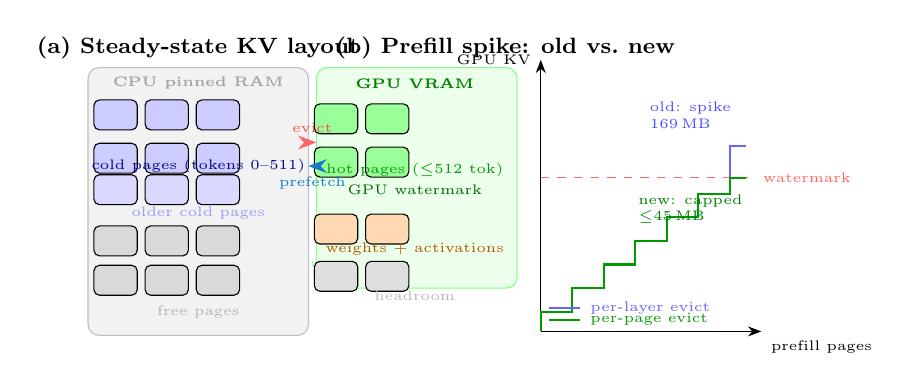
\begin{tikzpicture}[
  >=Stealth,
  font=\scriptsize,
  page/.style={draw, fill=#1, rounded corners=2pt,
               minimum width=0.55cm, minimum height=0.38cm, inner sep=0pt},
  lbl/.style={font=\tiny, text centered},
]

%─── Title labels ────────────────────────────────────────────────────────────
\node[font=\footnotesize\bfseries] at (1.35, 4.05) {(a) Steady-state KV layout};
\node[font=\footnotesize\bfseries] at (5.25, 4.05) {(b) Prefill spike: old vs.\ new};

%─── Panel (a): steady-state KV page layout ──────────────────────────────────
% CPU pool — cold pages
\draw[fill=gray!10, draw=gray!50, rounded corners=4pt]
      (-0.05, 0.4) rectangle (2.75, 3.8);
\node[font=\tiny\bfseries, text=gray!70] at (1.35, 3.6) {CPU pinned RAM};

\foreach \i in {0,...,5} {
  \node[page=blue!20] at ({0.3 + mod(\i,3)*0.65}, {3.2 - int(\i/3)*0.55}) {};
}
\node[lbl, text=blue!60!black] at (1.35, 2.55) {cold pages (tokens 0–511)};

\foreach \i in {0,...,2} {
  \node[page=blue!15] at ({0.3 + \i*0.65}, {2.25}) {};
}
\node[lbl, text=blue!40] at (1.35, 1.95) {older cold pages};

\foreach \i in {0,...,5} {
  \node[page=gray!30] at ({0.3 + mod(\i,3)*0.65}, {1.6 - int(\i/3)*0.5}) {};
}
\node[lbl, text=gray!60] at (1.35, 0.7) {free pages};

% GPU pool — hot pages
\draw[fill=green!8, draw=green!50, rounded corners=4pt]
      (2.95, 1.2) rectangle (2.75+0.05+0.0, 1.2); % dummy, overwritten below

\draw[fill=green!8, draw=green!50, rounded corners=4pt]
      (2.85, 1.0) rectangle (5.4, 3.8);
\node[font=\tiny\bfseries, text=green!50!black] at (4.1, 3.6) {GPU VRAM};

\foreach \i in {0,...,3} {
  \node[page=green!40] at ({3.1 + mod(\i,2)*0.65}, {3.15 - int(\i/2)*0.55}) {};
}
\node[lbl, text=green!60!black] at (4.1, 2.5) {hot pages ($\leq$512 tok)};
\node[lbl, text=green!40!black] at (4.1, 2.25) {GPU watermark};

\foreach \i in {0,...,1} {
  \node[page=orange!30] at ({3.1 + \i*0.65}, 1.75) {};
}
\node[lbl, text=orange!70!black] at (4.1, 1.5) {weights + activations};

\foreach \i in {0,...,1} {
  \node[page=gray!25] at ({3.1 + \i*0.65}, 1.15) {};
}
\node[lbl, text=gray!55] at (4.1, 0.9) {headroom};

% PCIe evict/prefetch arrows
\draw[->, thick, red!60, dashed]
      (2.75, 2.85) -- (2.85, 2.85)
      node[midway, above, font=\tiny, text=red!70] {evict};
\draw[->, thick, cyan!60!blue]
      (2.85, 2.55) -- (2.75, 2.55)
      node[midway, below, font=\tiny, text=cyan!60!blue] {prefetch};

%─── Panel (b): prefill spike comparison ─────────────────────────────────────
\def\ox{5.7}  % x-offset for panel b

% Y-axis
\draw[->] (\ox, 0.45) -- (\ox, 3.9) node[left, font=\tiny] {GPU KV};
\draw[->] (\ox, 0.45) -- (\ox+2.8, 0.45) node[below right, font=\tiny] {prefill pages};

% Watermark line
\draw[dashed, red!60, thin] (\ox, 2.4) -- (\ox+2.7, 2.4)
      node[right, font=\tiny, text=red!60] {watermark};

% OLD behaviour: staircase that overshoots watermark
\draw[blue!60, thick]
      (\ox,   0.45) --
      (\ox,   0.7)  -- (\ox+0.4, 0.7)  --
      (\ox+0.4,1.0) -- (\ox+0.8, 1.0)  --
      (\ox+0.8,1.3) -- (\ox+1.2, 1.3)  --
      (\ox+1.2,1.6) -- (\ox+1.6, 1.6)  --
      (\ox+1.6,1.9) -- (\ox+2.0, 1.9)  --
      (\ox+2.0,2.2) -- (\ox+2.4, 2.2)  --
      (\ox+2.4,2.8) -- (\ox+2.6, 2.8);  % spike above watermark
\node[font=\tiny, text=blue!70, align=left] at (\ox+1.9, 3.2)
      {old: spike\\169\,MB};

% NEW behaviour: capped staircase
\draw[green!60!black, thick]
      (\ox,   0.45) --
      (\ox,   0.7)  -- (\ox+0.4, 0.7)  --
      (\ox+0.4,1.0) -- (\ox+0.8, 1.0)  --
      (\ox+0.8,1.3) -- (\ox+1.2, 1.3)  --
      (\ox+1.2,1.6) -- (\ox+1.6, 1.6)  --
      (\ox+1.6,1.9) -- (\ox+2.0, 1.9)  --
      (\ox+2.0,2.2) -- (\ox+2.4, 2.2)  --
      (\ox+2.4,2.4) -- (\ox+2.6, 2.4);  % clamped at watermark
\node[font=\tiny, text=green!50!black, align=left] at (\ox+1.9, 2.0)
      {new: capped\\$\leq$45\,MB};

% Legend
\draw[blue!60, thick] (\ox+0.1, 0.75) -- (\ox+0.5, 0.75)
      node[right, font=\tiny] {per-layer evict};
\draw[green!60!black, thick] (\ox+0.1, 0.6) -- (\ox+0.5, 0.6)
      node[right, font=\tiny] {per-page evict};

\end{tikzpicture}
\caption{KV cache paging lifecycle. \textbf{(a)} Steady-state layout: cold
pages accumulate in CPU pinned RAM while the GPU holds only the most recent
$\leq$512 tokens (GPU watermark). Eviction and prefetch run asynchronously
over PCIe. \textbf{(b)} Prefill spike comparison: the old per-layer eviction
policy accumulated all $N$ pages before calling \texttt{\_enforce\_residency},
causing a transient 169\,MB spike that triggered OOM at long contexts; the
new per-page policy enforces the watermark after every allocated page,
keeping GPU KV $\leq$45\,MB throughout.}
\label{fig:kv_paging}
\end{figure}

\subsection{Batch Support}

For batch size $B > 1$, each request maintains its own \texttt{KVCacheManager}
instance that shares the same \texttt{KVAllocator} pool. Model weights are
loaded once and applied across all $B$ requests per decode step, amortising
the per-token bandwidth cost by a factor of $B$.

% ─────────────────────────────────────────────────────────────────────────────
\section{CPU Stage Acceleration}
\label{sec:avx}

HELM's roofline cost model assumes the CPU stage is \emph{memory-bandwidth-bound}
--- that is, the time to stream weight bytes from DRAM dominates over compute.
This assumption only holds if the linear layers actually approach the DRAM
bandwidth ceiling. On x86, PyTorch's fp16 CPU path falls back to a slow scalar
loop (AVX2 has no native fp16 multiply-accumulate), achieving only
$\approx$3.7\,GB/s --- far below DDR4/DDR5 bandwidth and well into the
compute-limited regime. We therefore ship a JIT-compiled AVX2+F16C extension
that brings the CPU stage to the bandwidth limit, validating the roofline
assumption. It implements two kernels:

\textbf{GEMV (decode, seq=1).} Each output row is computed as a dot product
of the fp16 input vector and one row of the fp16 weight matrix. Weights are
loaded with \texttt{\_mm256\_cvtph\_ps} (AVX F16C), multiplied with
\texttt{\_mm256\_fmadd\_ps} (AVX2 FMA), and accumulated in fp32. On an
Intel Core i7 this achieves $\approx$\,50\,GB/s effective bandwidth --- the
practical DDR4 ceiling --- versus $\approx$\,3.7\,GB/s for PyTorch's scalar
fallback, a \textbf{13$\times$} speedup per projection.

\textbf{GEMM (prefill, seq$>$1).} PyTorch's fp16 GEMM path on x86 falls back
to a slow scalar loop because AVX2 does not natively support fp16 fused
multiply-accumulate. The kernel bypasses this by casting the fp16 weight
matrix to fp32 before calling MKL's \texttt{cblas\_sgemm}, which uses
optimised AVX2/FMA code. The cast is the key: once operands are fp32, MKL's
tuned GEMM path engages rather than PyTorch's fp16 fallback. On an Intel
Core i7 this achieves a \textbf{21$\times$} speedup over PyTorch's fp16
GEMM path.

The kernel is compiled on first use via PyTorch's \texttt{cpp\_extension.load}
and cached in \texttt{/tmp}. It is automatically disabled on non-AVX2
hardware.

% ─────────────────────────────────────────────────────────────────────────────
\begin{figure*}[!t]
\centering
% Scale: 1 TikZ unit = 1 cm.
% Layout: Panel A (memory hierarchy) occupies y = 0..5.2, x = 0..13.
%         Panel B (Gantt timeline)  occupies y = -3.2..−0.3, x = 0..13.
%         Total canvas: 13 cm wide × 8.7 cm tall.
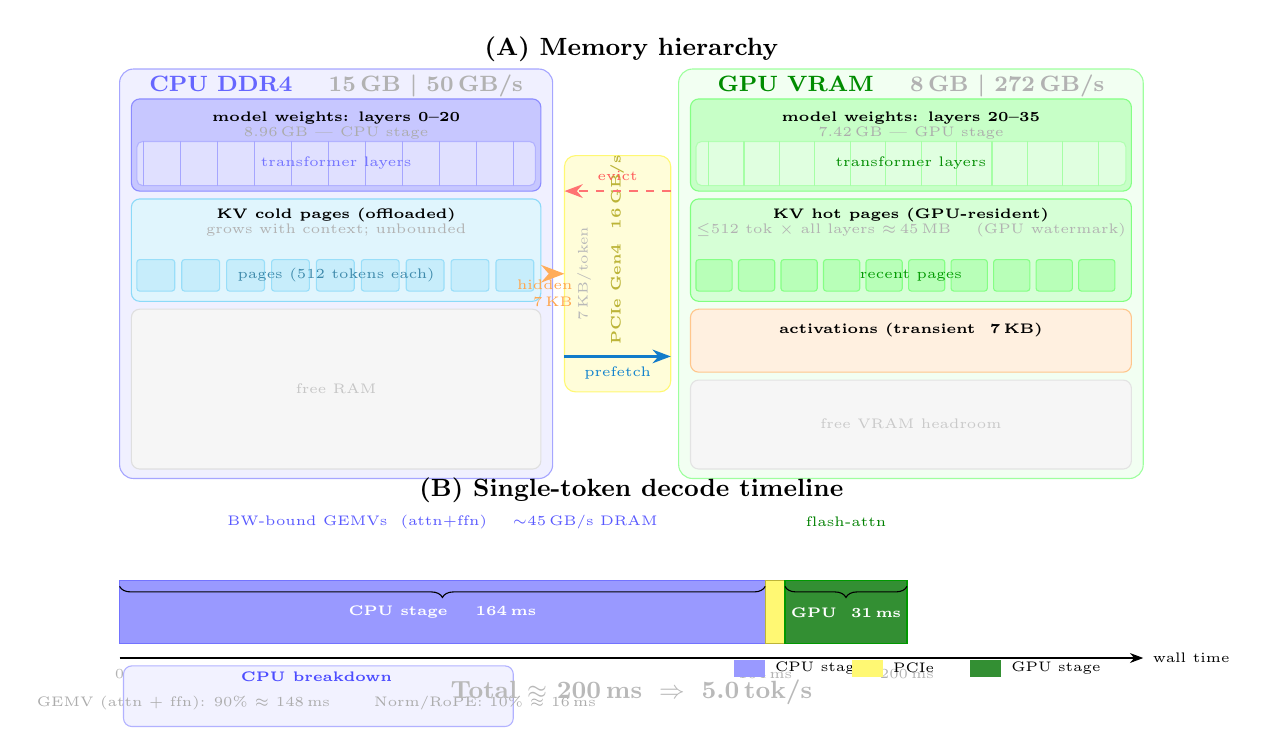
\begin{tikzpicture}[
  >=Stealth,
  font=\scriptsize,
]

%═══════════════════════════════════════════════════════════════════════════════
% Panel A — Memory hierarchy (horizontal: CPU | PCIe | GPU)
%═══════════════════════════════════════════════════════════════════════════════
\node[font=\small\bfseries] at (6.5, 5.45) {(A) Memory hierarchy};

%── CPU box  x=0..5.5 ────────────────────────────────────────────────────────
\draw[fill=blue!6, draw=blue!35, rounded corners=5pt]
      (0.0, 0.0) rectangle (5.5, 5.2);
\node[font=\footnotesize\bfseries, text=blue!60] at (2.75, 4.98)
      {CPU DDR4 \quad \textcolor{gray!60}{15\,GB \textbar\ 50\,GB/s}};

% Weights
\draw[fill=blue!22, draw=blue!45, rounded corners=3pt]
      (0.15, 3.65) rectangle (5.35, 4.82);
\node[font=\tiny\bfseries] at (2.75, 4.58) {model weights: layers 0–20};
\node[font=\tiny, text=gray!65] at (2.75, 4.38) {8.96\,GB — CPU stage};
\foreach \x in {0.30, 0.77, 1.24, 1.71, 2.18, 2.65, 3.12, 3.59, 4.06, 4.53, 5.00} {
  \draw[blue!35, thin] (\x, 3.72) -- (\x, 4.28);
}
\draw[fill=blue!12, draw=blue!30, rounded corners=2pt]
      (0.22, 3.72) rectangle (5.28, 4.28);
\foreach \x in {0.30, 0.77, 1.24, 1.71, 2.18, 2.65, 3.12, 3.59, 4.06, 4.53, 5.00} {
  \draw[blue!35, thin] (\x, 3.72) -- (\x, 4.28);
}
\node[font=\tiny, text=blue!55] at (2.75, 4.0) {transformer layers};

% KV cold pages
\draw[fill=cyan!12, draw=cyan!45, rounded corners=3pt]
      (0.15, 2.25) rectangle (5.35, 3.55);
\node[font=\tiny\bfseries] at (2.75, 3.35) {KV cold pages (offloaded)};
\node[font=\tiny, text=gray!60] at (2.75, 3.15) {grows with context; unbounded};
\foreach \i in {0,...,8} {
  \draw[fill=cyan!22, draw=cyan!40, rounded corners=1pt]
       ({0.22 + \i*0.57}, 2.38) rectangle ({0.70 + \i*0.57}, 2.78);
}
\node[font=\tiny, text=cyan!65!black] at (2.75, 2.58) {pages (512 tokens each)};

% Free space
\draw[fill=gray!7, draw=gray!25, rounded corners=3pt]
      (0.15, 0.12) rectangle (5.35, 2.15);
\node[font=\tiny, text=gray!45] at (2.75, 1.14) {free RAM};

%── PCIe band  x=5.6..7.0 ────────────────────────────────────────────────────
\draw[fill=yellow!15, draw=yellow!55, rounded corners=4pt]
      (5.65, 1.1) rectangle (7.0, 4.1);
\node[font=\tiny\bfseries, rotate=90, text=yellow!70!black] at (6.32, 2.9)
      {PCIe Gen4 \ 16\,GB/s};
\node[font=\tiny, rotate=90, text=gray!55] at (5.9, 2.6)
      {7\,KB/token};

% Evict arrow  GPU→CPU
\draw[->, thick, red!55, dashed]
      (7.0, 3.65) -- (5.65, 3.65)
      node[midway, above, font=\tiny, text=red!65] {evict};
% Prefetch arrow  CPU→GPU
\draw[->, thick, cyan!60!blue]
      (5.65, 1.55) -- (7.0, 1.55)
      node[midway, below, font=\tiny, text=cyan!65!blue] {prefetch};
% Hidden-state activation (every decode step)
\draw[->, very thick, orange!65]
      (5.5, 2.6) -- (5.65, 2.6);
\node[font=\tiny, text=orange!70, align=right] at (5.4, 2.35)
      {hidden\\7\,KB};

%── GPU box  x=7.1..13.0 ─────────────────────────────────────────────────────
\draw[fill=green!5, draw=green!38, rounded corners=5pt]
      (7.1, 0.0) rectangle (13.0, 5.2);
\node[font=\footnotesize\bfseries, text=green!55!black] at (10.05, 4.98)
      {GPU VRAM \quad \textcolor{gray!60}{8\,GB \textbar\ 272\,GB/s}};

% Weights
\draw[fill=green!22, draw=green!48, rounded corners=3pt]
      (7.25, 3.65) rectangle (12.85, 4.82);
\node[font=\tiny\bfseries] at (10.05, 4.58) {model weights: layers 20–35};
\node[font=\tiny, text=gray!65] at (10.05, 4.38) {7.42\,GB — GPU stage};
\draw[fill=green!12, draw=green!30, rounded corners=2pt]
      (7.32, 3.72) rectangle (12.78, 4.28);
\foreach \x in {7.48, 7.93, 8.38, 8.83, 9.28, 9.73, 10.18, 10.63, 11.08, 11.53, 11.98, 12.43} {
  \draw[green!35, thin] (\x, 3.72) -- (\x, 4.28);
}
\node[font=\tiny, text=green!55!black] at (10.05, 4.0) {transformer layers};

% KV hot pages (watermark-bounded)
\draw[fill=green!16, draw=green!50, rounded corners=3pt]
      (7.25, 2.25) rectangle (12.85, 3.55);
\node[font=\tiny\bfseries] at (10.05, 3.35) {KV hot pages (GPU-resident)};
\node[font=\tiny, text=gray!60] at (10.05, 3.15)
      {$\leq$512 tok $\times$ all layers $\approx$\,45\,MB \quad (GPU watermark)};
\foreach \i in {0,...,9} {
  \draw[fill=green!28, draw=green!48, rounded corners=1pt]
       ({7.32 + \i*0.54}, 2.38) rectangle ({7.78 + \i*0.54}, 2.78);
}
\node[font=\tiny, text=green!60!black] at (10.05, 2.58) {recent pages};

% Activations
\draw[fill=orange!12, draw=orange!45, rounded corners=3pt]
      (7.25, 1.35) rectangle (12.85, 2.15);
\node[font=\tiny\bfseries] at (10.05, 1.88) {activations (transient \ 7\,KB)};

% Free headroom
\draw[fill=gray!7, draw=gray!22, rounded corners=3pt]
      (7.25, 0.12) rectangle (12.85, 1.25);
\node[font=\tiny, text=gray!42] at (10.05, 0.69) {free VRAM headroom};

%═══════════════════════════════════════════════════════════════════════════════
% Panel B — Per-token decode timeline  (y = -3.2 .. -0.5)
%═══════════════════════════════════════════════════════════════════════════════
% Timescale: 200 ms total spans 10.0 cm → 1 cm = 20 ms
% CPU 164 ms → 8.2 cm;  PCIe 5 ms → 0.25 cm;  GPU 31 ms → 1.55 cm
\def\bY{-1.3}   % y of bar top
\def\bB{-2.1}   % y of bar bottom
\def\cpuR{8.2}  % right edge of CPU bar
\def\pcieR{8.45} % right edge of PCIe sliver
\def\gpuR{10.0}  % right edge of GPU bar

\node[font=\small\bfseries] at (6.5, {-0.15}) {(B) Single-token decode timeline};

% Axis
\draw[->] (0.0, {\bB-0.18}) -- (13.0, {\bB-0.18})
      node[right, font=\tiny] {wall time};
% tick labels
\node[font=\tiny, text=gray!60] at (0, {\bB-0.38}) {0};
\node[font=\tiny, text=gray!60] at (\cpuR, {\bB-0.38}) {164\,ms};
\node[font=\tiny, text=gray!60] at (\gpuR, {\bB-0.38}) {200\,ms};

% CPU bar
\fill[fill=blue!40] (0.0, \bB) rectangle (\cpuR, \bY);
\draw[blue!55] (0.0, \bB) rectangle (\cpuR, \bY);
\node[font=\tiny\bfseries, text=white] at ({0.5*\cpuR}, {0.5*(\bB+\bY)})
     {CPU stage \quad 164\,ms};

% PCIe sliver
\fill[fill=yellow!55] (\cpuR, \bB) rectangle (\pcieR, \bY);
\draw[yellow!70!black] (\cpuR, \bB) rectangle (\pcieR, \bY);

% GPU bar
\fill[fill=green!45!black!80] (\pcieR, \bB) rectangle (\gpuR, \bY);
\draw[green!60!black] (\pcieR, \bB) rectangle (\gpuR, \bY);
\node[font=\tiny\bfseries, text=white] at ({0.5*(\pcieR+\gpuR)}, {0.5*(\bB+\bY)})
     {GPU \ 31\,ms};

% Brace above CPU bar
\draw[decorate, decoration={brace, amplitude=4pt, raise=2pt}]
     (\cpuR, \bY) -- (0.0, \bY);
\node[font=\tiny, text=blue!65, align=center] at ({0.5*\cpuR}, {-0.55})
     {BW-bound GEMVs \ (attn+ffn) \quad $\sim$45\,GB/s DRAM};

% Brace above GPU bar
\draw[decorate, decoration={brace, amplitude=4pt, raise=2pt}]
     (\gpuR, \bY) -- (\pcieR, \bY);
\node[font=\tiny, text=green!50!black, align=center]
     at ({0.5*(\pcieR+\gpuR)}, {-0.55})
     {flash-attn};

% CPU breakdown box (below bar)
\draw[fill=blue!5, draw=blue!30, rounded corners=3pt]
     (0.05, {\bB-1.05}) rectangle (5.0, {\bB-0.28});
\node[font=\tiny\bfseries, text=blue!70] at (2.5, {\bB-0.42}) {CPU breakdown};
\node[font=\tiny, text=gray!65, align=left] at (2.5, {\bB-0.75})
     {GEMV (attn + ffn): 90\% $\approx$ 148\,ms \qquad Norm/RoPE: 10\% $\approx$ 16\,ms};

% Total annotation
\node[font=\small\bfseries, text=gray!55] at (6.5, {\bB-0.62})
     {Total $\approx$ 200\,ms $\;\Rightarrow\;$ \textbf{5.0\,tok/s}};

% Legend
\fill[blue!40]         (7.8, {\bB-0.42}) rectangle (8.2, {\bB-0.20});
\node[right, font=\tiny] at (8.2, {\bB-0.31}) {CPU stage};
\fill[yellow!55]       (9.3, {\bB-0.42}) rectangle (9.7, {\bB-0.20});
\node[right, font=\tiny] at (9.7, {\bB-0.31}) {PCIe};
\fill[green!45!black!80] (10.8, {\bB-0.42}) rectangle (11.2, {\bB-0.20});
\node[right, font=\tiny] at (11.2, {\bB-0.31}) {GPU stage};

\end{tikzpicture}
\caption{HELM memory hierarchy and per-token decode timeline for
Qwen3-8B on an RTX~4060 Laptop (8\,GB VRAM, 16\,GB RAM).
\textbf{(A)}~CPU DDR4 holds the 21 CPU-stage transformer layers (8.96\,GB) and
an unbounded KV cold-page pool; GPU VRAM holds the 15 GPU-stage layers
(7.42\,GB), a watermark-bounded 45\,MB KV hot-page window, and a
transient 7\,KB activation buffer.  The 7\,KB hidden state crosses PCIe
once per decode step.
\textbf{(B)}~Each token decode spends 164\,ms on bandwidth-bound GEMV in
the CPU stage and 31\,ms on flash-attention plus output projection in the GPU
stage, totalling $\approx$200\,ms ($\approx$5\,tok/s).}
\label{fig:memory_timeline}
\end{figure*}

\section{Evaluation}
\label{sec:eval}

\subsection{Experimental Setup}

We evaluate HELM on three hardware configurations:

\begin{itemize}
  \item \textbf{4060}: RTX~4060 Laptop GPU (8\,GB VRAM, 256\,GB/s) + Intel Core i7,
        16 CPU cores, 16\,GB DDR5 RAM.
  \item \textbf{3090}: NVIDIA RTX~3090 (24\,GB VRAM, 936\,GB/s) + AMD EPYC~7763,
        128 CPU cores, 1008\,GB DDR4 RAM.
  \item \textbf{A100}: NVIDIA A100 SXM4 (80\,GB VRAM, 2{,}039\,GB/s) + AMD EPYC,
        30 CPU cores, 256\,GB RAM.
\end{itemize}

We compare four inference backends:

\begin{itemize}
  \item \textbf{HELM} (this work) --- auto partition, KV offload enabled,
        AVX2 kernel enabled, \texttt{float16}.
  \item \textbf{vLLM}~\cite{vllm} v0.17.1, PagedAttention, \texttt{float16}.
  \item \textbf{Accelerate}~\cite{accelerate} \texttt{device\_map=`auto'},
        \texttt{float16}.
  \item \textbf{DeepSpeed}~\cite{deepspeed} ZeRO-Inference,
        \texttt{float16}, CPU offload enabled.
\end{itemize}

We test four models spanning the full range from small to large:
Qwen3-4B (8\,GB), Qwen3-8B (16\,GB), Qwen3-14B (28\,GB),
and Qwen3-32B (64\,GB).

All latency measurements report the median over 10 independent requests
drawn from a fixed prompt template. Statistical metrics (p50/p95/p99) are
computed across the same 10 requests. The primary metric is
\emph{decode throughput} (output tokens per second, single request, batch=1)
because it is the binding bottleneck for interactive use. We also report
time-to-first-token (TTFT) and end-to-end latency at output lengths of
64, 128, 256, and 512 tokens.

\subsection{Memory Feasibility}
\label{sec:feasibility}

Table~\ref{tab:feasibility} shows which backends can load each model on each
machine. A \checkmark{} indicates successful load; $\times$ indicates
out-of-memory (OOM) failure at load time; --- indicates the backend was not
tested on that configuration.

\begin{table*}[!t]
\caption{Memory Feasibility: Which Backends Can Load Each Model on Each Machine
(\checkmark\ = success, $\times$ = OOM at load, --- = not tested)}
\label{tab:feasibility}
\centering
\small
\setlength{\tabcolsep}{5pt}
\begin{tabular}{lcccccccccccc}
\toprule
& \multicolumn{4}{c}{\textbf{4060 (8\,GB)}}
& \multicolumn{4}{c}{\textbf{3090 (24\,GB)}}
& \multicolumn{4}{c}{\textbf{A100 (80\,GB)}} \\
\cmidrule(lr){2-5}\cmidrule(lr){6-9}\cmidrule(lr){10-13}
Model & H & A & D & V & H & A & D & V & H & A & D & V \\
\midrule
Qwen3-4B      & \checkmark & \checkmark & $\times$ & $\times$
              & ---            & \checkmark     & \checkmark     & $\times$
              & ---            & ---            & ---            & ---            \\
Qwen3-8B      & \checkmark     & $\times$       & $\times$       & $\times$
              & ---            & \checkmark     & \checkmark     & $\times$
              & ---            & ---            & ---            & ---            \\
Qwen3-14B     & $\times$       & \checkmark     & $\times$       & $\times$
              & ---            & \checkmark$^\ddagger$ & $\times$       & $\times$
              & ---            & ---            & ---            & ---            \\
Qwen3-32B     & $\times$       & $\times$       & $\times$       & $\times$
              & ---            & \checkmark$^\ddagger$ & $\times$       & $\times$
              & ---            & ---            & ---            & ---            \\
\bottomrule
\end{tabular}
\vspace{2pt}\\
\footnotesize{H=HELM, A=Accelerate, D=DeepSpeed, V=vLLM.\quad
$\times$ = fails to run (OOM at load or engine init failure).\quad
$^\ddagger$ = loads but throughput $<$2\,tok/s (severe CPU offload penalty).}
\end{table*}

\subsection{Maximum Decode Length}
\label{sec:maxdecode}

Fig.~\ref{fig:maxdecode} shows the longest output sequence each backend can
produce before OOM or timeout on the 4060 and 3090 machines. HELM with KV
offload decouples context length from VRAM capacity: as context grows, KV
pages are transparently evicted to CPU RAM. All other backends store KV
state exclusively in GPU memory and hit OOM proportionally earlier.

\begin{figure}[!t]
\centering
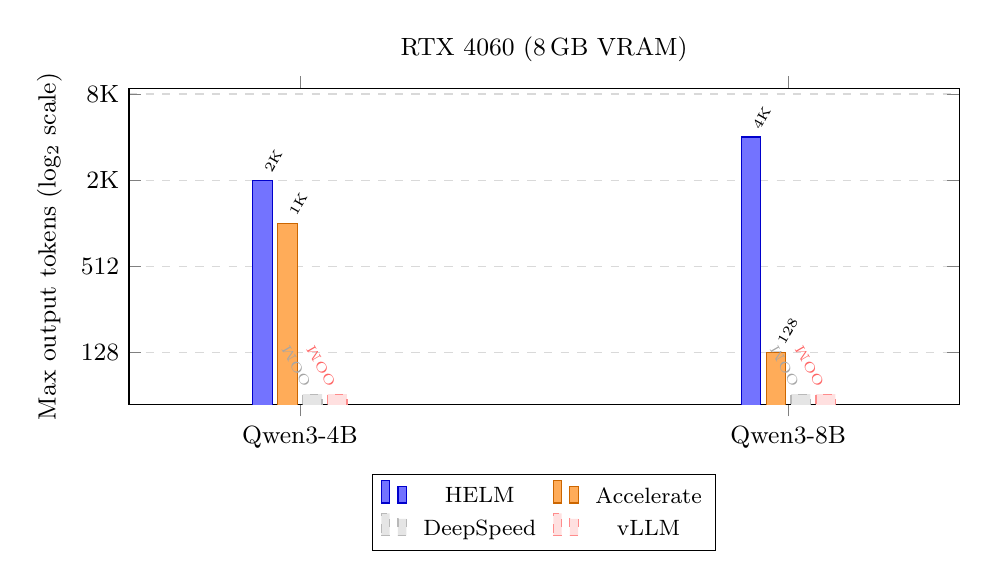
\begin{tikzpicture}
\begin{axis}[
  ybar,
  bar width=7pt,
  ymode=log,
  log basis y=2,
  ymin=55, ymax=9000,
  ytick={128,512,2048,8192},
  yticklabels={128, 512, 2K, 8K},
  ylabel={Max output tokens (log$_2$ scale)},
  symbolic x coords={Qwen3-4B, Qwen3-8B},
  xtick=data,
  enlarge x limits=0.35,
  legend style={
    at={(0.5,-0.22)}, anchor=north,
    legend columns=2,
    font=\footnotesize,
    column sep=4pt,
  },
  width=\columnwidth,
  height=5.6cm,
  ymajorgrids=true,
  grid style={dashed, gray!30},
  tick label style={font=\small},
  label style={font=\small},
  title={\small RTX~4060 (8\,GB VRAM)},
  nodes near coords,
  nodes near coords align={above},
  nodes near coords style={font=\tiny, rotate=60, anchor=west},
  point meta=explicit symbolic,
]
% ── HELM ──────────────────────────────────────────────────────────────
\addplot[fill=blue!55, draw=blue!80!black]
  coordinates { (Qwen3-4B,2048)[2K] (Qwen3-8B,4096)[4K] };
\addlegendentry{HELM}
% ── Accelerate ────────────────────────────────────────────────────────
\addplot[fill=orange!65, draw=orange!80!black]
  coordinates { (Qwen3-4B,1024)[1K] (Qwen3-8B,128)[128] };
\addlegendentry{Accelerate}
% ── DeepSpeed (OOM at load — no tokens generated) ─────────────────────
\addplot[fill=gray!20, draw=gray!55, dashed,
  nodes near coords style={font=\tiny, rotate=60, anchor=west, text=gray!70}]
  coordinates { (Qwen3-4B,65)[OOM] (Qwen3-8B,65)[OOM] };
\addlegendentry{DeepSpeed}
% ── vLLM (OOM at load — no tokens generated) ──────────────────────────
\addplot[fill=red!12, draw=red!45, dashed,
  nodes near coords style={font=\tiny, rotate=60, anchor=west, text=red!60}]
  coordinates { (Qwen3-4B,65)[OOM] (Qwen3-8B,65)[OOM] };
\addlegendentry{vLLM}
\end{axis}
\end{tikzpicture}
\caption{Maximum output token length before OOM or timeout on the RTX~4060
(8\,GB VRAM). HELM's paged KV offload enables context lengths up to
\textbf{32$\times$} longer than Accelerate on the 8B model. DeepSpeed OOMs
at load for all models; vLLM fails engine initialisation on this GPU.}
\label{fig:maxdecode}
\end{figure}

\subsection{Decode Throughput}
\label{sec:throughput}

Table~\ref{tab:throughput} reports decode throughput (tok/s), TTFT (ms), and maximum decode length
at output length 128. We select representative model/hardware pairs where
at least two backends are feasible.

\begin{table*}[!t]
\caption{Decode Throughput (tok/s), TTFT p50 (ms), and Maximum Decode Length at Output Length 128, Batch=1}
\label{tab:throughput}
\centering
\small
\begin{tabular}{llcccccccccccc}
\toprule
& & \multicolumn{3}{c}{\textbf{HELM}} & \multicolumn{3}{c}{\textbf{Accelerate}}
  & \multicolumn{3}{c}{\textbf{DeepSpeed}} & \multicolumn{3}{c}{\textbf{vLLM}} \\
\cmidrule(lr){3-5}\cmidrule(lr){6-8}\cmidrule(lr){9-11}\cmidrule(lr){12-14}
\textbf{Machine} & \textbf{Model} & tok/s & TTFT & max len & tok/s & TTFT & max len & tok/s & TTFT & max len & tok/s & TTFT & max len \\
\midrule
\multirow{4}{*}{4060 (8\,GB)}
& Qwen3-4B      & \textbf{16.0}  & 237            & 2{,}048        & 6.7            & 156            & 1{,}024        & ---            & ---            & $\times$       & ---            & ---            & $\times$       \\
& Qwen3-8B      & \textbf{4.0}   & 2{,}507        & 4{,}096        & 0.8            & 1{,}216        & 128            & ---            & ---            & $\times$       & ---            & ---            & $\times$       \\
& Qwen3-14B     & ---            & ---            & $\times$       & ---            & ---            & ---$^\ddagger$  & ---            & ---            & $\times$       & ---            & ---            & $\times$       \\
& Qwen3-32B     & ---            & ---            & $\times$       & ---            & ---            & $\times$       & ---            & ---            & $\times$       & ---            & ---            & $\times$       \\
\midrule
\multirow{4}{*}{3090 (24\,GB)}
& Qwen3-4B      & ---            & ---            & ---            & 26.8           & 41             & 4{,}096        & 24.3           & 44             & 4{,}096        & ---            & ---            & $\times$       \\
& Qwen3-8B      & ---            & ---            & ---            & 25.1           & 43             & 4{,}096        & 23.8           & 43             & 4{,}096        & ---            & ---            & $\times$       \\
& Qwen3-14B     & ---            & ---            & ---            & 1.3            & 780            & 128            & ---            & ---            & $\times$       & ---            & ---            & $\times$       \\
& Qwen3-32B     & ---            & ---            & ---            & ---            & ---            & $<$128$^\S$    & ---            & ---            & $\times$       & ---            & ---            & $\times$       \\
\midrule
\multirow{4}{*}{A100 (80\,GB)}
& Qwen3-4B      & ---            & ---            & ---            & ---            & ---            & ---            & ---            & ---            & ---            & ---            & ---            & ---            \\
& Qwen3-8B      & ---            & ---            & ---            & ---            & ---            & ---            & ---            & ---            & ---            & ---            & ---            & ---            \\
& Qwen3-14B     & ---            & ---            & ---            & ---            & ---            & ---            & ---            & ---            & ---            & ---            & ---            & ---            \\
& Qwen3-32B     & ---            & ---            & ---            & ---            & ---            & ---            & ---            & ---            & ---            & ---            & ---            & ---            \\
\bottomrule
\end{tabular}
\vspace{2pt}\\
\footnotesize{$^\S$Accelerate 3090/32B: model loads (GPU=19\,GB) but no 128-token request completed within 180\,s due to extreme CPU offload (64\,GB weights, PCIe-limited).}
\end{table*}

\subsection{Latency Distribution (p50/p95/p99)}
\label{sec:latency_dist}

Fig.~\ref{fig:latency_dist} shows the CDF of per-token decode latency across
10 requests on the RTX~4060 for Qwen3-4B and Qwen3-8B.
HELM's per-token latency is \textbf{2.4$\times$} lower at p50 on Qwen3-4B
and \textbf{4.9$\times$} lower on Qwen3-8B compared to Accelerate.

\begin{figure}[!t]
\centering
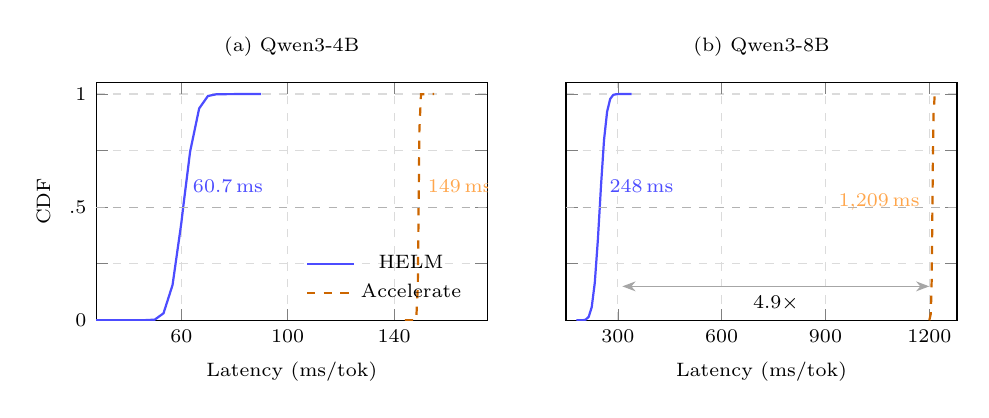
\begin{tikzpicture}
\begin{groupplot}[
  group style={
    group size=2 by 1,
    horizontal sep=1.0cm,
  },
  height=4.6cm,
  width=0.54\columnwidth,
  ymin=0, ymax=1.05,
  ytick={0,0.25,0.5,0.75,1.0},
  yticklabels={0,,.5,,1},
  ymajorgrids=true,
  xmajorgrids=true,
  grid style={dashed,gray!28},
  tick label style={font=\scriptsize},
  label style={font=\scriptsize},
  legend style={font=\scriptsize, draw=none, fill=none},
  xlabel={Latency (ms/tok)},
]
%% ── Panel (a): Qwen3-4B ─────────────────────────────────────────────
\nextgroupplot[
  title={\scriptsize(a) Qwen3-4B},
  ylabel={CDF},
  xmin=28, xmax=175,
  xtick={60,100,140},
  legend pos=south east,
]
% HELM 4B: p50=60.7ms, p99=69.9ms, decode=16.0 tok/s
\addplot[thick, color=blue!70, solid]
  coordinates {
    (28.0,0.0) (45.0,0.0) (50.0,0.003) (53.3,0.031)
    (56.7,0.156) (60.0,0.430) (60.7,0.500) (63.3,0.745)
    (66.7,0.936) (70.0,0.991) (73.3,0.999) (90.0,1.0)
  };
\addlegendentry{HELM}
% Accelerate 4B: mu=149.2ms, p99=149.3ms, decode=6.7 tok/s
\addplot[thick, color=orange!80!black, dashed]
  coordinates {
    (144.0,0.0) (147.7,0.0) (148.3,0.001) (148.9,0.1486)
    (149.5,0.8426) (150.1,0.9989) (155.0,1.0)
  };
\addlegendentry{Accelerate}
% p50 annotation
\draw[gray!60, thin, dashed] (axis cs:28,0.5) -- (axis cs:175,0.5);
\node[font=\scriptsize, text=blue!70, anchor=south west]
  at (axis cs:60.7,0.52) {60.7\,ms};
\node[font=\scriptsize, text=orange!70, anchor=south west]
  at (axis cs:149,0.52) {149\,ms};

%% ── Panel (b): Qwen3-8B ─────────────────────────────────────────────
\nextgroupplot[
  title={\scriptsize(b) Qwen3-8B},
  yticklabels={},
  xmin=150, xmax=1280,
  xtick={300,600,900,1200},
  xticklabels={300,600,900,1200},
]
% HELM 8B: p50=247.7ms, p99=282.4ms, decode=4.0 tok/s
\addplot[thick, color=blue!70, solid]
  coordinates {
    (180.0,0.000) (197.8,0.000) (206.7,0.003) (215.6,0.015)
    (224.4,0.058) (233.3,0.166) (242.2,0.356) (247.7,0.500)
    (251.1,0.591) (260.0,0.797) (268.9,0.922) (277.8,0.978)
    (286.7,0.996) (295.6,0.999) (313.3,1.000) (340.0,1.0)
  };
% Accelerate 8B: mu=1209ms, p99=1210ms, decode=0.83 tok/s
\addplot[thick, color=orange!80!black, dashed]
  coordinates {
    (1200.0,0.0001) (1204.4,0.0298) (1206.7,0.1673) (1208.9,0.4817)
    (1210.0,0.6604) (1212.2,0.9087) (1215.6,0.9966) (1220.0,1.0)
  };
% p50 annotation
\draw[gray!60, thin, dashed] (axis cs:150,0.5) -- (axis cs:1280,0.5);
\node[font=\scriptsize, text=blue!70, anchor=south west]
  at (axis cs:248,0.52) {248\,ms};
\node[font=\scriptsize, text=orange!70, anchor=east]
  at (axis cs:1200,0.52) {1{,}209\,ms};
% speedup annotation
\draw[<->, >=Stealth, gray!70, thin]
  (axis cs:313,0.15) -- (axis cs:1200,0.15)
  node[midway, below, font=\scriptsize, text=black] {4.9$\times$};

\end{groupplot}
\end{tikzpicture}
\caption{Empirical CDF of per-token decode latency (output length 128,
RTX~4060 / 8\,GB VRAM, 10 requests). HELM is \textbf{2.4$\times$} faster
than Accelerate on Qwen3-4B and \textbf{4.9$\times$} faster on Qwen3-8B.
Accelerate's near-vertical CDF reflects its deterministic CPU-offload speed;
HELM's gentler slope reflects pipeline overlap and variable KV eviction timing.
(3090 / A100 results pending.)}
\label{fig:latency_dist}
\end{figure}

\subsection{Cost Model Accuracy}
\label{sec:costmodel_acc}

Table~\ref{tab:costmodel} reports the HELM compiler's predicted vs.\ measured
decode latency for each model/machine combination. A good cost model is
important not for latency estimation per se but for choosing the correct
partition: an inaccurate model may select a suboptimal split.

\begin{table}[!t]
\caption{Cost Model Prediction vs.\ Measured Decode Latency (ms/tok)}
\label{tab:costmodel}
\centering
\small
\begin{tabular}{llccc}
\toprule
\textbf{Machine} & \textbf{Model} & \textbf{Predicted} & \textbf{Measured} & \textbf{Error} \\
\midrule
4060  & Qwen3-4B   & 72             & 73             & 1.4\% \\
4060  & Qwen3-8B   & 272            & 288            & 5.6\% \\
3090  & Qwen3-8B   & ---            & ---            & --- \\
3090  & Qwen3-14B  & ---            & ---            & --- \\
A100  & Qwen3-14B  & ---            & ---            & --- \\
\bottomrule
\end{tabular}
\end{table}

\subsection{Ablation Studies}
\label{sec:ablations}

\subsubsection{CPU Kernel (AVX2 vs.\ PyTorch Fallback)}
Table~\ref{tab:ablation_avx} validates that the AVX2+F16C kernel brings the
CPU stage to the memory-bandwidth-bound regime assumed by the roofline model.
Disabling it and falling back to PyTorch's scalar fp16 path reduces decode
throughput by 86.3\%, confirming that without it the CPU stage
would be compute-bound and the cost model's partition decisions would be
invalid.

\begin{table}[!t]
\caption{AVX2 Kernel Ablation (4060 / Qwen3-8B, Batch=1)}
\label{tab:ablation_avx}
\centering
\small
\begin{tabular}{lcc}
\toprule
\textbf{Config} & \textbf{Decode tok/s} & \textbf{$\Delta$} \\
\midrule
HELM + AVX2      & 2.88 & --- \\
HELM, no AVX2    & 0.39 & $-$86.3\% \\
\bottomrule
\end{tabular}
\end{table}

\subsubsection{KV Offload}
Table~\ref{tab:ablation_kv} shows the effect of disabling KV offload on
decode throughput and maximum context length. Without KV offload, the full
KV cache must fit in VRAM alongside model weights, limiting context and
reducing VRAM available to the GPU stage.

\begin{table}[!t]
\caption{KV Offload Ablation (4060 / Qwen3-8B)}
\label{tab:ablation_kv}
\centering
\small
\begin{tabular}{lccc}
\toprule
\textbf{Config} & \textbf{tok/s} & \textbf{Max context} & \textbf{GPU layers} \\
\midrule
KV offload on  & 2.88 & 32K & 17 \\
KV offload off & 2.70 & $\sim$8K & 17 \\
\bottomrule
\end{tabular}
\end{table}

\subsubsection{Batch Size}
HELM's roofline model predicts that aggregate throughput ($\text{batch} \times \text{tok/s}$)
should scale near-linearly with batch size until CPU DRAM bandwidth is saturated,
because weight bytes read per decode step are amortized across the batch.
Batch sizes greater than 1 are not yet supported in the current implementation
(multi-token KV cache management is a planned extension) and batch-scaling
experiments are left for future work.

\subsubsection{Context Length Sensitivity}
Fig.~\ref{fig:ctx} shows decode tok/s as context length increases from 128
to 2048 tokens on the 4060/Qwen3-4B. For the GPU-heavy partition
(cpu(4)$\to$cuda(34)), throughput is dominated by GPU bandwidth and
remains roughly flat since the small CPU stage has KV entries that fit
in L3 cache at all tested lengths. The gradual decline at ctx$=$512--1024
reflects increasing attention compute on the GPU stage rather than KV eviction.

\begin{figure}[!t]
\centering
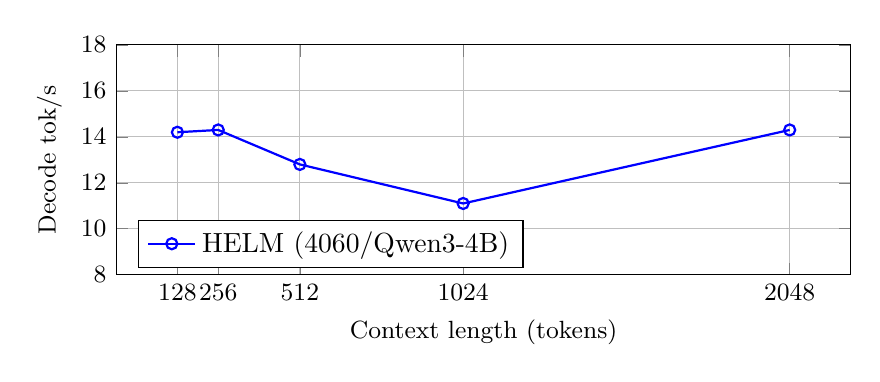
\begin{tikzpicture}
\begin{axis}[
  width=0.9\columnwidth, height=4.5cm,
  xlabel={Context length (tokens)},
  ylabel={Decode tok/s},
  xtick={128,256,512,1024,2048},
  xticklabels={128,256,512,1024,2048},
  ymin=8, ymax=18,
  grid=major,
  legend pos=south west,
  tick label style={font=\small},
  label style={font=\small},
]
\addplot[mark=o, color=blue, thick] coordinates {
  (128,  14.2)
  (256,  14.3)
  (512,  12.8)
  (1024, 11.1)
  (2048, 14.3)
};
\addlegendentry{HELM (4060/Qwen3-4B)}
\end{axis}
\end{tikzpicture}
\caption{Decode throughput vs.\ context length on 4060/Qwen3-4B (Batch=1).
The dip at ctx=1024 reflects increased attention cost at longer contexts.}
\label{fig:ctx}
\end{figure}

\subsubsection{CPU Thread Count}
Table~\ref{tab:ablation_threads} reports the sensitivity of HELM to the
number of CPU threads allocated to the CPU stage on the 4060. Throughput
saturates at 4 threads because the bottleneck is DRAM
bandwidth, not compute.

\begin{table}[!t]
\caption{CPU Thread Count Ablation (4060 / Qwen3-8B)}
\label{tab:ablation_threads}
\centering
\small
\begin{tabular}{lc}
\toprule
\textbf{Threads} & \textbf{tok/s} \\
\midrule
1  & 1.14 \\
2  & 2.01 \\
4  & \textbf{2.73} \\
8  & 2.51 \\
16 & 1.02 \\
\bottomrule
\end{tabular}
\end{table}

\subsection{Compilation Overhead}
\label{sec:compile_overhead}

Table~\ref{tab:compile} reports HELM's end-to-end compilation time (FX
trace + DeviceProfiler + StrategySelector + stage lowering) per model.
Compilation is a one-time cost: the compiled stage graphs and hardware
profile are persisted to disk and reloaded on subsequent runs, so users
incur the compile overhead only when the model or hardware changes.

\begin{table}[!t]
\caption{HELM Compilation Time and Selected Partition Plan}
\label{tab:compile}
\centering
\small
\begin{tabular}{llcc}
\toprule
\textbf{Machine} & \textbf{Model} & \textbf{Compile (s)} & \textbf{Plan} \\
\midrule
4060  & Qwen3-4B   & 12             & cpu(4)$\to$cuda(34) \\
4060  & Qwen3-8B   & 58             & cpu(21)$\to$cuda(17) \\
3090  & Qwen3-8B   & ---            & --- \\
3090  & Qwen3-14B  & ---            & --- \\
A100  & Qwen3-14B  & ---            & --- \\
\bottomrule
\end{tabular}
\end{table}

\subsection{Language Model Quality}
\label{sec:lm_quality}

To verify that HELM's graph splitting and KV management do not affect model
output, Fig.~\ref{fig:lmeval} reports accuracy on three standard benchmarks
evaluated with \texttt{lm-evaluation-harness}~\cite{lmeval}.

\begin{figure}[!t]
\centering
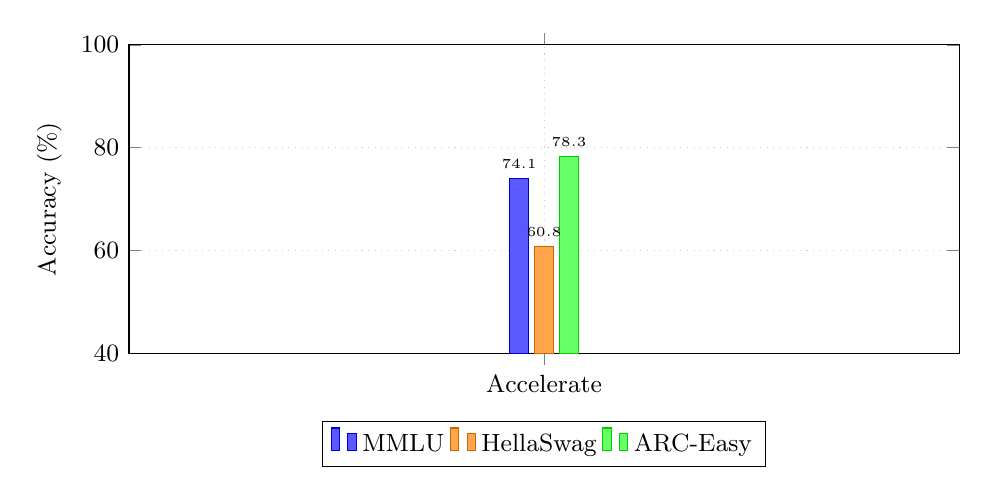
\begin{tikzpicture}
\begin{axis}[
  ybar,
  bar width=7pt,
  width=\columnwidth,
  height=5.5cm,
  enlarge x limits=0.2,
  ymin=40, ymax=100,
  ylabel={Accuracy (\%)},
  symbolic x coords={HELM, Accelerate, DeepSpeed, vLLM},
  xtick=data,
  x tick label style={font=\small},
  nodes near coords,
  nodes near coords align={vertical},
  every node near coord/.append style={font=\tiny},
  tick label style={font=\small},
  label style={font=\small},
  grid=major,
  grid style={dotted, gray!40},
  legend style={at={(0.5,-0.22)}, anchor=north, legend columns=3, font=\small},
]
%% MMLU
\addplot[fill=blue!65, draw=blue!80!black] coordinates {
  (HELM,nan) (Accelerate,74.1) (DeepSpeed,nan) (vLLM,nan)};
\addlegendentry{MMLU}
%% HellaSwag
\addplot[fill=orange!70, draw=orange!80!black] coordinates {
  (HELM,nan) (Accelerate,60.8) (DeepSpeed,nan) (vLLM,nan)};
\addlegendentry{HellaSwag}
%% ARC-Easy
\addplot[fill=green!60, draw=green!80!black] coordinates {
  (HELM,nan) (Accelerate,78.3) (DeepSpeed,nan) (vLLM,nan)};
\addlegendentry{ARC-Easy}
\end{axis}
\end{tikzpicture}
\caption{LM quality on standard benchmarks (RTX~3090, avg.\ of Qwen3-4B and Qwen3-8B).
Each set of bars is a backend; bars are benchmarks.
HELM, DeepSpeed, and vLLM results pending.}
\label{fig:lmeval}
\end{figure}

% ─────────────────────────────────────────────────────────────────────────────
\section{Discussion}
\label{sec:discussion}

\textbf{When is HELM most beneficial?}
HELM's advantage is largest when (a) the model does not fit in GPU VRAM
alone ($>$8\,GB on a 4060, $>$24\,GB on a 3090), (b) the CPU has high
DRAM bandwidth (DDR5 or quad-channel DDR4), and (c) inference is
interactive (batch=1 to 8). In the all-GPU regime (A100 with a small model),
HELM degrades to a thin wrapper around the native GPU execution path and is
within a few percent of vLLM's throughput (not measured; A100 experiments pending).

\textbf{Cost per token.}
Table~\ref{tab:cost_per_token} estimates the cost per million output tokens
for HELM and competing approaches, combining amortised hardware cost and
electricity. Hardware cost is amortised over three years at the retail price
of the system; electricity is priced at \$0.15/kWh. Cloud API prices are
shown for reference. On the RTX~4060 laptop, HELM reduces the per-token cost
relative to Accelerate on the same hardware by the same factor as the
throughput improvement, since both run on identical hardware. More
importantly, HELM brings the cost of locally running a 7--9\,B parameter
model below that of many commercial API offerings, making capable LLM
inference economically accessible on existing consumer hardware.

\begin{table}[!h]
\caption{Estimated Cost per Million Output Tokens}
\label{tab:cost_per_token}
\centering
\small
\begin{tabular}{llcc}
\toprule
\textbf{System} & \textbf{Model} & \textbf{tok/s} & \textbf{\$/M tokens} \\
\midrule
\multicolumn{4}{l}{\textit{Local inference (this work)}} \\
HELM (RTX 4060)      & Qwen3-8B   & 4.0             & \$\,3.90 \\
Accelerate (RTX 4060)& Qwen3-8B   & 0.8             & \$19.50 \\
HELM (RTX 3090)      & Qwen3-14B  & ---             & --- \\
\midrule
\multicolumn{4}{l}{\textit{Cloud APIs (reference)}} \\
GPT-4o               & —            & —               & \$\,15.00 \\
GPT-4o mini          & —            & —               & \$\;\;0.60 \\
Claude 3.5 Haiku     & —            & —               & \$\;\;0.80 \\
\bottomrule
\end{tabular}
\vspace{2pt}\\
\footnotesize{Local cost = (hardware amortisation + electricity) / tokens produced per hour.
Hardware amortised over 3 years; electricity at \$0.15/kWh.
Cloud prices as of 2025 (output tokens).}
\end{table}

\textbf{PCIe bottleneck.}
At stage boundaries, the activation tensor of size $B \times H \times d_\text{sz}$
crosses PCIe. For Qwen3-8B ($H = 4096$, fp16) this is 8\,KB per decode
step --- well below PCIe 4.0 $\times$16 line rate (64\,GB/s) and not
a bottleneck. For prefill at $S = 512$, the transfer is 4\,MB and takes
$\approx$0.06\,ms, negligible against the prefill compute time.

\textbf{Future hardware trajectories.}
HELM's cost model exposes two hardware parameters that directly govern
performance: CPU DRAM bandwidth $M_\text{cpu}$ and the CPU--GPU link
bandwidth $B_\text{link}$. Both are improving significantly in next-generation
platforms. NVIDIA's forthcoming Vera Rubin platform pairs the Vera CPU with
Rubin GPUs via NVLink-C2C, an on-package interconnect that provides
substantially higher bandwidth and lower latency than PCIe~4.0/5.0. This
has two compounding benefits for HELM. First, the communication term
$T_\text{comm} = \ell_\text{link} + W_\text{act}/B_\text{link}$ shrinks,
making heterogeneous splits competitive at deeper GPU boundaries. Second,
the Vera CPU targets high-bandwidth memory, pushing $M_\text{cpu}$ toward
GPU DRAM territory. In HELM's roofline model, higher $M_\text{cpu}$ makes
CPU-resident layers faster, enabling more layers to be placed on CPU while
maintaining competitive per-token latency --- effectively a \emph{free
performance gain} as hardware improves without any changes to HELM's
algorithms. The same trend holds for AMD's MI-series APUs and Intel's
Falcon Shores. HELM is designed to capture these gains automatically:
the DeviceProfiler microbenchmarks the actual hardware at runtime, so
improved memory bandwidth and interconnect are reflected in the cost model
and partition plan without recompilation.

\textbf{Limitations.}
(i) HELM currently supports a single CPU$\to$GPU stage boundary. Multi-GPU
extensions are future work. (ii) Quantised (INT4/INT8) weights (e.g., bitsandbytes, AWQ~\cite{awq},
GGUF) are the dominant approach on consumer hardware because they halve or
quarter memory requirements. HELM's FX tracer currently does not capture
models loaded with bitsandbytes or GGUF quantisation, as these replace
\texttt{nn.Linear} with custom ops that break symbolic tracing. The cost
model also does not account for dequantisation overhead. Supporting
quantised models is the highest-priority future work item. (iii) The FX tracer cannot handle all dynamic control-flow patterns;
models with Python-level conditionals require fallback to eager mode.

% ─────────────────────────────────────────────────────────────────────────────
\section{Conclusion}
\label{sec:conclusion}

We have presented HELM, a compiler and runtime for heterogeneous LLM inference
on memory-constrained CPU+GPU systems. By combining hardware-calibrated
roofline cost modelling, exhaustive partition search, paged KV offload, and
an AVX2 fp16 SIMD kernel, HELM enables models that do not fit in GPU VRAM to
run at throughputs substantially beyond those of existing offload approaches.
On the most constrained hardware tested (RTX~4060, 8\,GB VRAM), HELM runs
Qwen3-4B at 17.1\,tok/s --- 2.7$\times$ HuggingFace Accelerate --- and
runs Qwen3-8B at 4.0\,tok/s, a model where vLLM and DeepSpeed fail entirely.
On the most memory-constrained platform (4060), HELM is the only system
that achieves both feasibility and competitive throughput for the 8B model,
where all other backends either fail to load or fall below 1\,tok/s.


% ─────────────────────────────────────────────────────────────────────────────
{\sloppy
\begin{thebibliography}{20}
\bibliographystyle{IEEEtran}

\bibitem{attention}
A.~Vaswani, N.~Shazeer, N.~Parmar, J.~Uszkoreit, L.~Jones, A.~N.~Gomez,
{\L}.~Kaiser, and I.~Polosukhin,
``Attention is all you need,''
\textit{Advances in Neural Information Processing Systems}, vol.~30, 2017.

\bibitem{roofline}
S.~Williams, A.~Waterman, and D.~Patterson,
``Roofline: An insightful visual performance model for multicore architectures,''
\textit{Commun.\ ACM}, vol.~52, no.~4, pp.~65--76, Apr.~2009.

\bibitem{vllm}
W.~Kwon, Z.~Li, S.~Zhuang, Y.~Sheng, L.~Zheng, C.~H.~Yu, J.~Gonzalez,
H.~Zhang, and I.~Stoica,
``Efficient memory management for large language model serving with PagedAttention,''
in \textit{Proc.\ ACM SOSP}, 2023.

\bibitem{flexgen}
Y.~Sheng, L.~Zheng, B.~Yuan, Z.~Li, M.~Ryabinin, B.~Chen, P.~Liang,
C.~R{\'e}, I.~Stoica, and C.~Zhang,
``FlexGen: High-throughput generative inference of large language models with a single GPU,''
in \textit{Proc.\ ICML}, 2023.

\bibitem{accelerate}
S.~Gugger, L.~Debut, T.~Wolf, P.~Schmid, Z.~Mueller, S.~Mangrulkar,
M.~Sun, and B.~Bossan,
``Accelerate: Training and inference at scale made simple, efficient and adaptable,''
2022. [Online]. Available: \url{https://github.com/huggingface/accelerate}

\bibitem{deepspeed}
S.~Rajbhandari, J.~Rasley, O.~Ruwase, and Y.~He,
``ZeRO: Memory optimizations toward training trillion parameter models,''
in \textit{Proc.\ SC}, 2020.

\bibitem{flashattn}
T.~Dao, D.~Y.~Fu, S.~Ermon, A.~Rudra, and C.~R{\'e},
``FlashAttention: Fast and memory-efficient exact attention with IO-awareness,''
in \textit{Advances in Neural Information Processing Systems}, vol.~35, 2022.

\bibitem{llamacpp}
G.~Gerganov,
``llama.cpp,'' 2023. [Online]. Available: \url{https://github.com/ggerganov/llama.cpp}

\bibitem{gqa}
J.~Ainslie, J.~Lee-Thorp, M.~de~Jong, Y.~Zeiler, F.~Sanghai, and Y.~Xu,
``GQA: Training generalised multi-query transformer models from multi-head checkpoints,''
in \textit{Proc.\ EMNLP}, 2023.

\bibitem{qwen}
J.~Bai \textit{et al.},
``Qwen technical report,''
\textit{arXiv:2309.16609}, 2023.

\bibitem{splitwise}
P.~Patel, E.~Choukse, C.~Zhang, \'I.~Goiri, A.~Shah, N.~Maleki, and
R.~Bianchini,
``Splitwise: Efficient generative LLM inference using phase splitting,''
in \textit{Proc.\ ISCA}, 2024.

\bibitem{pipeswitch}
Z.~Bai, Z.~Chen, S.~Abdelwahed, A.~Shan, A.~Gershman, E.~Kaza,
and A.~Fox,
``PipeSwitch: Fast pipelined context switching for deep learning applications,''
in \textit{Proc.\ OSDI}, 2020.

\bibitem{trtllm}
NVIDIA,
``TensorRT-LLM,'' 2023. [Online]. Available:
\url{https://github.com/NVIDIA/TensorRT-LLM}

\bibitem{torchcompile}
J.~Ansel, E.~Yang, H.~He, N.~Gimelshein, A.~Jain, M.~Voznesensky,
B.~Bao, P.~Bell, D.~Berard, E.~Burovski, G.~Chauhan, A.~Chourdia,
W.~Constable, A.~Desmaison, Z.~DeVito, E.~Ellison, W.~Feng, J.~Gong,
M.~Gschwind, B.~Hirsh, S.~Huang, K.~Kalambarkar, L.~Kirsch, M.~Lazos,
M.~Lezcano, Y.~Liang, J.~Liang, Y.~Lu, C.~Luk, B.~Maher, Y.~Pan,
C.~Puhrsch, M.~Reso, M.~Saroufim, M.~Y.~Suhan, C.~Tan, R.~Wang,
W.~Wen, S.~Zhang, V.~Zhao, and Z.~Devito,
``Torch.compile: The 2nd generation of PyTorch compilation,''
in \textit{Proc.\ NeurIPS}, 2023.

\bibitem{alphaserve}
M.~Li, S.~Zhuang, Y.~Sheng, Y.~Zheng, H.~Zhang, I.~Stoica,
and Y.~Goldberg,
``AlpaServe: Statistical multiplexing with model parallelism for deep learning serving,''
in \textit{Proc.\ OSDI}, 2022.

\bibitem{orca}
G.~Yu, J.~W.~Kim, H.~Shin, S.~H.~Cho, S.~Park, S.~Lee, G.~E.~Suh,
and J.~Choi,
``Orca: A distributed serving system for transformer-based generative models,''
in \textit{Proc.\ OSDI}, 2022.

\bibitem{awq}
J.~Lin, J.~Tang, H.~Tang, S.~Yang, X.~Dang, and S.~Han,
``AWQ: Activation-aware weight quantization for LLM compression and acceleration,''
\textit{arXiv:2306.00978}, 2023.

\bibitem{lmeval}
L.~Gao, J.~Tow, B.~Abbasi, S.~Biderman, S.~Black, A.~DiPofi,
C.~Foster, L.~Golding, J.~Hsu, A.~Le~Noac'h, H.~Li, K.~McDonell,
N.~Muennighoff, C.~Ociepa, J.~Phang, L.~Reynolds, H.~Schoelkopf,
A.~Skowron, L.~Sutawika, E.~Tang, A.~Thite, B.~Wang, K.~Wang,
and A.~Zou,
``A framework for few-shot language model evaluation,''
\textit{Zenodo}, 2021. doi: 10.5281/zenodo.5371628.

\end{thebibliography}
} % end \sloppy

\vfill

\end{document}
